\documentclass[table,mathserif,12pt]{beamer}% notheorems,

\usepackage{xeCJK}         % CJK 中文支持
\setCJKmainfont{SourceHanSerifSC-Medium}
\setmainfont{Times New Roman}  

% $Header: /cvsroot/latex-beamer/latex-beamer/solutions/generic-talks/generic-ornate-15min-45min.en.tex,v 1.4 2004/10/07 20:53:08 tantau Exp $

%\usepackage[width=2cm,dark,tab]{beamerthemesidebar}
%\usepackage{colortbl} % ��ɫ����
%\usepackage[table]{xcolor}
%\usepackage{booktabs} % ����ʹ�����߱�
%\usepackage{multirow} % ���ӱ���ʹ��multirow������ظ�package
%\usepackage{dcolumn}
\usepackage{graphicx,subfigure,boxedminipage}
\usepackage{bm}
\usepackage{amsmath}
\usepackage[english]{babel}
% or whatever
\usepackage{CJK}
\usepackage[latin1]{inputenc}
% or whatever
\usepackage{alltt}
\usepackage{amsmath,amssymb,amsfonts}
\usepackage{times}
\usepackage{multimedia}
\usepackage{color}% [usenames]
\usepackage{hyperref}
%\usepackage[T1]{fontenc}
\graphicspath {{figure/}}%ͼƬ���ڵ�Ŀ¼
\usepackage{multicol}    %ͬʱʹ�õ��кͶ��У�����
%%%\begin{multicols}{2}
%%%\end{multicols}
\usepackage{setspace} % �������
%\begin{spacing}{1.5}
%\tableofcontents \listoffigures \listoftables
%\end{spacing}

\setlength{\columnsep}{-0.05cm} %˫��֮��ļ��
%\setlength{\parskip}{-0.1\baselineskip} % ���öμ��


\mode<presentation> {
  \usetheme{Antibes}   %[hideothersubsections] beamer ģ���ģʽ
  % Warsaw or ...,Antibes,PaloAlto,Darmstadt,Frankfurt,Boadilla,Antibes,Luebeck,CambridgeUS,Rochester

%%  With navigation bar: default, boxes, Bergen, Madrid, Pittsburgh, Rochester
%%  With a treelike navigation bar: Antibes, JuanLesPins, Montpellier.
%%  With a TOC sidebar: Berkeley, PaloAlto, Goettingen, Marburg, Hannover
%%  With a mini frame navigation: Berlin, Ilmenau, Dresden, Darmstadt, Frankfurt, Singapore, Szeged
%%  With section and subsection titles: Copenhagen, Luebeck, Malmoe, Warsaw



%  \usefonttheme[onlylarge]{structuresmallcapsserif}%
%  \usefonttheme[onlysmall]{structurebold}%
%  \usefonttheme{serif} % Times New Rome ����
  \usecolortheme{sidebartab}% default
%% Inner color themes, ����ѡ��: orchid,albatross,beaver,beetle,default,crane,dolphin,dove,fly,orchid,lily,rose,seagull,seahorse
%% Inner color themes, ����ѡ��: sidebartab,whale,wolverine

  \useinnertheme[shadow=true]{rounded} % default,circles,margin,rounded,rectangles
%%  \useoutertheme{split} % default��infolines��miniframes,shadow,smoothbars,smoothtree,tree,sidebar

%  \useoutertheme[height=0.1\textwidth,width=0.15\textwidth,hideothersubsections]{sidebar}
  \setbeamercovered{dynamic} % dynamic,transparent,invisible
  % or whatever (possibly just delete it)
}

%% beamer���Ѿ��������ɫ��
%% red,green,blue,cyan,magenty,yellow,black,darkgray,gray,lightgray,orange,violet,purple,brown

%% �Զ�����ɫ��
%% \xdefinecolor{lanvendar}{rgb}{0.8,0.6,1}
%% \xdefinecolor{olive}{cmyk}{0.64,0,0.95,0.4}
%% \colorlet{structure}{blue!60!black}
 \colorlet{structure}{blue!85!white}      %  �Զ�����ɫ,�á�structure����ʾ 60%��ɫ+40%��ɫ����ɫ


%\setbeamertemplate{background canvas}[vertical shading][bottom=white,top=structure.fg!25] %%����ɫ, ��25%����, ���ɵ��°�.
%\beamertemplateshadingbackground{white}{blue!25} %���ý���(gradient)����ɫ,
%\beamersetaveragebackground{yellow!25} % ���õ�һ��(solid)����ɫ
%\beamertemplategridbackground[0.3cm] % ����դ��(grid ) ����

\def\hilite<#1>{\temporal<#1>{\color{blue!80}}{\color{blue!85!white}}{\color{black}}}% magenta
%% �Զ�������, Դ�� beamer_guide. item ����ʾʱ, ʹ��Ҫ���ֵ�item��������ʾ��item���Ѿ����ֵ�item�� ���ֲ�ͬ��ɫ.

\hypersetup{pdfpagemode={FullScreen}} % Ĭ��ȫ������


% Or whatever. Note that the encoding and the font should match. If T1
% does not look nice, try deleting the line with the fontenc.


%\logo{\includegraphics[height=0.1\textwidth]{hfut_logo_red.pdf}} % ��logo

%\pgfdeclareimage[height=5cm]{logo}{ustc_logo_new.pdf}
%\logo{\pgfuseimage{logo}}

\setbeamertemplate{navigation symbols}{}   %% ȥ��ҳ���·�Ĭ�ϵĵ�����.
\setcounter{tocdepth}{2} % ֻ����2��Ŀ¼
\setcounter{secnumdepth}{2}
\numberwithin{equation}{section} % ��ʽ���±��
%\numberwithin{equation}{subsection} % ��ʽ���ڱ��
\numberwithin{figure}{section} % ͼƬ���±��

\renewcommand{\raggedright}{\leftskip=0pt \rightskip=0pt plus 0cm} %  ���˶���
\raggedright

\setbeamertemplate{caption}[numbered] % ͼ�����
\setbeamerfont{caption}{size=\footnotesize} %  ͼ�����������С����

%%%%%%%%%%%%%%%%%% ������һҳ����ռλ %%%%%%%%%%%%%%%%%%%%
 \defbeamertemplate*{frametitle}{smoothbars theme}
  {%
    \nointerlineskip%
    \begin{beamercolorbox}[wd=\paperwidth,leftskip=.3cm,rightskip=.3cm plus1fil,vmode]{frametitle}
      \vskip.6ex
      \usebeamerfont*{frametitle}\insertframetitle%
      \vskip.6ex
    \end{beamercolorbox}%
  }

%%%%%%%%%%%%%%%%%%%%%%%%%%%%%% �Զ���ҳ�� %%%%%%%%%%%%%%%%%%%%%%%%%%%%%%%%%
\usefoottemplate{\hbox{\tinycolouredline{structure!80!black}{
\color{white}{ \insertshortauthor} \hfill{\insertshortinstitute }
\hfill{\insertframenumber\,/ \inserttotalframenumber}
% \hfill{{\the\year}/{\the\month}/{\the\day}}
}}}

%%%%%%%%%%%%%%%%%%%%%%%%%%%%% ��������%%%%%%%%%%%%%%%%%%%%%%%%%%%%%%%%%%%%%
%\newcommand{\song}{\CJKfamily{song}}
%\newcommand{\hei}{\CJKfamily{hei}}
%\newcommand{\kai}{\CJKfamily{kai}}
%\newcommand{\fs}{\CJKfamily{fs}}

%%%%%%%%%%%%%%%%%%%%%%%%%%%%% ���Ļ��� %%%%%%%%%%%%%%%%%%%%%%%%%%%%%%%%%%%%%
%\newtheorem{theo}{{����}} % \begin{theo}  \end{theo}
%\newtheorem{prop}{{����}}
%\newtheorem{lem}{{����}}
%\newtheorem{corol}{{����}}[theorem]
%\newtheorem{def}{{����}}
%\newtheorem{exam}{{��}}

%%%%%%%%%%%%%%%%%%%%%%%%%%%%% ���������� %%%%%%%%%%%%%%%%%%%%%%%%%%%%%%%%%%
\setbeamertemplate{theorems}[numbered]
\newtheorem{exam}{Example}[section] % ���±��




\title[Antennas and Radio Wave Propagation\quad whatisit] % (optional, use only with long paper titles)
{ \textsc{Antennas and Radio Wave Propagation} }
%\title{Antennas and Radio Wave Propagation}


\author[XXX YYY] % (optional, use only with lots of authors)
{\quad\\  \large  XXX YYY \\ {\scriptsize Email: XXX@YYY.com}}

% - Use the \inst{?} command only if the authors have different
%   affiliation.
\institute[Department of Communication Engineering] % (optional, but mostly needed)
{Department of Communication Engineering}

%\date {\scriptsize{2008Äê12ÔÂ09ÈÕ}}
%% ÈÕÆÚ×Ô¶¯Éú³É
\date{\scriptsize{\today} }%{{\the\year}Äê{\the\month}ÔÂ{\the\day}ÈÕ}



% If you have a file called "university-logo-filename.xxx", where xxx
% is a graphic format that can be processed by latex or pdflatex,
% resp., then you can add a logo as follows:

%\pgfdeclareimage[height=0.5cm]{ustc_logo_new.pdf}{ustc_logo_new.pdf}
%\logo{\pgfuseimage{ustc_logo_new.pdf}}


% Delete this, if you do not want the table of contents to pop up at
% the beginning of each subsection:
%\AtBeginSection[] {
%  \begin{frame}<beamer>
%    \frametitle{Outline}
%    \tableofcontents[currentsection]
%  \end{frame}
%}
%
%\AtBeginSubsection[] {
%  \begin{frame}<beamer>
%    \frametitle{Outline}
%    \tableofcontents[currentsection,currentsubsection]
%  \end{frame}
%}


% If you wish to uncover everything in a step-wise fashion, uncomment
% the following command:

%\beamerdefaultoverlayspecification{<+->} % ÖðÐÐÏÔʾ


\begin{document}

%%%%%%%%%%%%%%%%%%%%%%%%%%%%%%%%%%%%%%%%%%%%%%%%%%%%%%%%%%%%%%%%%
\begin{frame} % ·âÃæ
  \vspace{0.5cm}
  \titlepage
  \hypertarget{beginning}{}
\end{frame}

%%%%%%%%%%%%%%%%%%%%%%%%%%%%%%%%%%%%%%%%%%%%%%%%%%%%%%%%%%%%%%%%%

\begin{frame}
\frametitle{\textsc{Preface}}
\begin{itemize}
\item\hilite<1> {\bf Prerequisites Ô¤Ð޿γÌ:}
    \begin{itemize}
    \item Electromagnetic Fields and Electromagnetic Waves
    \item Microwave Technique
    \end{itemize}\pause

\item\hilite<2> {\bf Textbook whatisit2:}
    \begin{itemize}
    \item Antennas: For All Applications (Third Edition), John D. Kraus and
    Ronald J. Marhefka, Electronic Industry Press, 2008.
    \end{itemize}\pause

\item\hilite<3> {\bf Reference Books whatisit:}
    \begin{itemize}
    \item Antenna Theory Analysis and Design (3rd.Edition), Constantine
    A. Balanis, John Wiley and Sons, Inc.
    \item ¡¶whatisit¡·£¬ËÎ¬ÕŽ¨»ª£¬»ÆÒ±±àÖø£¬Î÷°²µç×ӿƼ¼´óѧ³ö°æÉç
    \end{itemize}
\end{itemize}

\end{frame}

%%%%%%%%%%%%%%%%%%%%%%%%%%%%%%%%%%%%%%%%%%%%%%%%%%%%%%%%%%%%%%%%%

\begin{frame}
  \frametitle{\textsc{Contents}} \vspace{-0.3cm}
  \tableofcontents[hidesubsections]
  % You might wish to add the option[pausesections,subsection]
\end{frame}

%%%%%%%%%%%%%%%%%%%%%%%%%%%%%%%%%%%%%%%%%%%%%%%%%%%%%%%%%%%%%%%%%

\section[Introduction ����]{Introduction}\label{sec:1}

%%%%%%%%%%%%%%%%%%%%%%%%%%%%%% ����Ŀ¼ҳ %%%%%%%%%%%%%%%%%%%%%%%%%%%%%%%%%%%

\begin{frame}%<beamer>
    \frametitle{\textsc{Contents}} \vspace{-1.05cm}
    \begin{multicols}{2}
    %\begin{figure}
    \begin{minipage}[t]{0.55\textwidth}
    \tableofcontents[currentsection,hideallsubsections]
    % [currentsection,hideallsubsections][sectionstyle=show/shaded,subsectionstyle=show/shaded/hide]
    \end{minipage}

    \begin{minipage}[t]{0.55\textwidth}
    \vspace{0.44cm}
    \begin{spacing}{1.2} % ������� ��Ҫ\usepackage{setspace}
    \begin{itemize}
    \item\hyperlink{subsec:1-1}{History}
    \item\hyperlink{subsec:1-2}{Dimensions and Units}
    \item\hyperlink{subsec:1-3}{Symbols and Notes}
    \item\hyperlink{subsec:1-4}{EM Spectrum}
    \end{itemize}
    \end{spacing}
    \end{minipage}
    %\end{figure}
    \end{multicols}

\end{frame}

%%%%%%%%%%%%%%%%%%%%%%%%%%%%%%%%%%%%%%%%%%%%%%%%%%%%%%%%%%%%%%%%%
\subsection[History ��չ��ʷ]{History}\label{subsec:1-1}
%%%%%%%%%%%%%%%%%%%%%%%%%%%%%%%%%%%%%%%%%%%%%%%%%%%%%%%%%%%%%%%%%
\begin{frame}
\frametitle{\textsc{History}}\transsplitverticalin

\begin{itemize}
\item In 1886, Professor Heinrich Rudolph Hertz
demonstrated the first wireless electromagnetic system. He was able
to produce in his laboratory at a wavelength of 4 m a spark in the
gap of a transmitting $\lambda/2$ dipole which was then detected as
a spark in the gap of a nearby loop.

\begin{figure}
  \begin{center}
    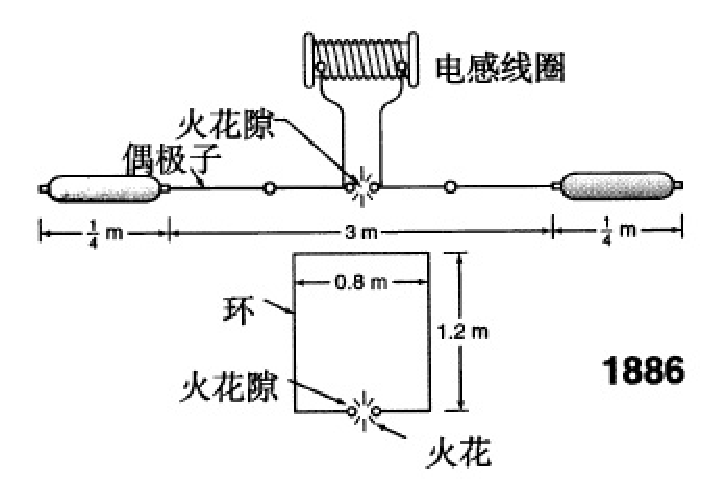
\includegraphics[scale=0.4]{ch1/first_radio_link} % ͼƬ�������Դ�Щ��ĸ��ͷ
  \end{center}
\end{figure}

\end{itemize}

\end{frame}

%%%%%%%%%%%%%%%%%%%%%%%%%%%%%%%%%%%%%%%%%%%%%%%%%%%%%%%%%%%%%%%%%
\begin{frame}
\frametitle{\textsc{History}}  \transsplitverticalout

\begin{itemize}
    \item In 1901, Guglielmo Marconi performed the first
    transatlantic transmission from Poldhu in Cornwall, England, to St.
    John's Newfoundland. This was the dawn of the antenna era.
    \begin{figure}
    \begin{center}
        \includegraphics[scale=0.5]{ch1/antenna_marconi} % ͼƬ�������Դ�Щ��ĸ��ͷ
    \end{center}
    \end{figure}
\end{itemize}

\end{frame}

%%%%%%%%%%%%%%%%%%%%%%%%%%%%%%%%%%%%%%%%%%%%%%%%%%%%%%%%%%%%%%%%%

\begin{frame}
\frametitle{\textsc{History}}%\transwipe % ͿĨЧ��

\begin{itemize}% [<+-| structure@+>]
\hilite<1>\item In 1940s, antenna technology was primarily centered
on wire related radiating elements and frequencies up to about UHF.
World War II launched a new era in antennas (such as waveguide
apertures, horns, reflectors).\pause

\hilite<2>\item 1960s-1990s, advances made in computer architecture
and technology have had a major impact on the advance of modern
antenna technology, numerical methods were introduced that allowed
previously intractable complex antenna system configurations to be
analyzed and designed very accurately.
\end{itemize}
\rightline{\hyperlink{sec:1}{\beamerreturnbutton{back}} }

\end{frame}

%%%%%%%%%%%%%%%%%%%%%%%%%%%%%%%%%%%%%%%%%%%%%%%%%%%%%%%%%%%%%%%%%
\subsection[Dimensions and Units ���ٺ͵�λ]{Dimensions and Units}\label{subsec:1-2}
%%%%%%%%%%%%%%%%%%%%%%%%%%%%%%%%%%%%%%%%%%%%%%%%%%%%%%%%%%%%%%%%%

\begin{frame}
\frametitle{\textsc{Dimensions and Units}} %\transwipe % ͿĨЧ��
\begin{itemize}
\hilite<1>\item A dimension defines some physical characteristic.
There are 7 fundamental dimensions: length, mass, time, electric
current, temperature, luminous intensity and amount of substance,
represented as $L,M,T,I,\mathcal{T},\mathcal{I},N$
���ٶ���ijЩ��������������������7����\pause

\hilite<2>\item A unit is a standard or reference by which a
dimension can be expressed numerically.
��λ��ʹ�����ܽ�����ֵ������һ�ֱ�׼����ա�\pause

\hilite<3>\item In the SI system, there are 7 fundamental units:
meter, kilogram, second, ampere, kelvin, candela, and mole for the 7
fundamental dimensions.
���ʵ�λ������7��������λ���ף�ǧ�ˣ��룬���࣬�����ģ���������Ħ����
% ������7���������ٳ��ȡ�������ʱ�䡢����ǿ�ȡ��¶ȡ�����ǿ�Ⱥ������Ļ�����λ��
\end{itemize}

\end{frame}

%%%%%%%%%%%%%%%%%%%%%%%%%%%%%%%%%%%%%%%%%%%%%%%%%%%%%%%%%%%%%%%%%

\begin{frame}
\frametitle{\textsc{Dimensions and Units}} %\transwipe % ͿĨЧ��
\begin{itemize}
\hilite<1>\item Second(s): duration of 9,192,631,770 periods of
radiation corresponding to the transition between two hyperfine
levels of the ground state of cesium-133.
�-133��̬����������ϸ�ܼ�֮����ǰ���Ӧ�ķ������ڵ�9,192,631,770��\pause

\hilite<2>\item Meter(m): path length traveled by light in vacuum in
a time $t=1/299,792,458$ second.
��������д���$t=1/299,792,458$����������·�̳��ȡ�\pause

\hilite<3>\item Kilogram(kg): the mass of the international
prototype kilogram, a cylinder of platinum-iridium alloy kept at
S\`{e}vres, France.
���ڱ����ڷ���������˹�IJ�ҿ�Ͻ��������ǧ��ԭ����������

\end{itemize}

\end{frame}

%%%%%%%%%%%%%%%%%%%%%%%%%%%%%%%%%%%%%%%%%%%%%%%%%%%%%%%%%%%%%%%%%

\begin{frame}
\frametitle{\textsc{Dimensions and Units}} %\transwipe % ͿĨЧ��
\begin{itemize}
\hilite<1>\item Ampere(A): the electric current flowing in each of
two infinitely long parallel wires in vacuum separated by 1m which
produces a force of 200 nanonewtons per meter of length
($200\rm{nNm}^{-1}=2\times10^{-7}\rm{Nm}^{-1}$).
������������1�׵����޳�ƽ�е�����ͨ���ĵ���������ʹ��������֮�����������������200��ţ��/�ס�\pause

\hilite<2>\item Kelvin(K): temperature equal to 1/273.16 of the
triple point of water. �¶ȵ���ˮ��������1/273.16��

\end{itemize}

\end{frame}

%%%%%%%%%%%%%%%%%%%%%%%%%%%%%%%%%%%%%%%%%%%%%%%%%%%%%%%%%%%%%%%%%

\begin{frame}
\frametitle{\textsc{Dimensions and Units}} %\transwipe % ͿĨЧ��
\begin{itemize}

\hilite<1>\item Candela(cd): luminous intensity equal to that of
1/600,000 $\rm m^2$ of a perfect radiator at the temperature of
freezing platinum at a pressure of 1 standard atmosphere.
�ڱ�׼����ѹ�Ͳ��������¶��£���������������1/600,000ƽ���׵Ĺ��նȡ�\pause

\hilite<2>\item Mole(mol): an amount of a substance that contains as
many elementary entities as there are atoms in 12 grams of pure
carbon-12 ($\rm{C}^{12}$). This corresponds to a value of
$6.02214179(30)\times10^{23}$. 12��̼-12��������ԭ������
\end{itemize}
\rightline{\hyperlink{sec:1}{\beamerreturnbutton{back}} }

\end{frame}

%%%%%%%%%%%%%%%%%%%%%%%%%%%%%%%%%%%%%%%%%%%%%%%%%%%%%%%%%%%%%%%%%
\subsection[Symbols and Notes ���źͼǺ�]{Symbols and Notes}\label{subsec:1-3}
%%%%%%%%%%%%%%%%%%%%%%%%%%%%%%%%%%%%%%%%%%%%%%%%%%%%%%%%%%%%%%%%%

\begin{frame}
\frametitle{\textsc{Symbols and Notes}}\transwipe % ͿĨЧ��
\vspace{-0.5cm}

{\footnotesize
\begin{table}[!h]
\rowcolors{1}{blue!20}{blue!10} \arrayrulecolor{blue!5}
\tabcolsep 4pt % ��
\renewcommand\arraystretch{1.1} % ��

\caption{Metric prefix}\label{tab:prefix} \vspace*{-15pt}
\begin{center}
    \setlength{\arrayrulewidth}{1.3pt}
%    \def\temptablewidth{0.95\textwidth}
%    {\rule{\temptablewidth}{1pt}}
    \begin{tabular}{c|c|c|c|c}%{\temptablewidth}{@{\extracolsep{\fill}}|c|c|c|c|c|}
        \arrayrulecolor{black}\hline
        \rowcolor{blue!50} Numerical value & Prefix & Symbol &
        U.S. Meaning & Chinese Meaning  \\   \hline
        $10^{18}$ & exa & E & quintillion & �� \\
        $10^{15}$ & peta & P & quadrillion & �� \\
        $10^{12}$ & era & T & trillion & ̫ \\
        $10^{9}$ & giga & G & billion & �� \\
        $10^{6}$ & mega & M & million & �� \\
        $10^{3}$ & kilo & k & thousand & ǧ \\
        $10^{-3}$ & milli & m & thousandth & �� \\
        $10^{-6}$ & micro & $\mu$ & millionth & ΢ \\
        $10^{-9}$ & nano & n & billionth & �� \\
        $10^{-12}$ & pico & p & trillionth & Ƥ \\
        $10^{-15}$ & femto & f & quadrillionth & �� \\
        $10^{-18}$ & atto & a & quintillionth & �� \\
        \hline
       \end{tabular}
%       {\rule{\temptablewidth}{1pt}}
\end{center}
\end{table}
}
\end{frame}

%%%%%%%%%%%%%%%%%%%%%%%%%%%%%%%%%%%%%%%%%%%%%%%%%%%%%%%%%%%%%%%%%

\begin{frame}
\frametitle{\textsc{Symbols and Notes}}%\transwipe % ͿĨЧ��
{\small
%\begin{block}{Example 1-1} % alartbloke
%\hspace{2em}$\mathbf{D}=\mathbf{\hat{x}}200\rm pCm^{-2}$\\
%means that the electric flux density $\mathbf{D}$ is a vector in the
%positive \textit{x} direction with a magnitude of 200 picocoulombs
%per square meter ($=200\times10^{-10}$ coulombs per square meter).
%��ͨ���ܶȣ�ʸ����Ϊ��x����200Ƥ����ÿƽ���ס�
%\end{block} \pause

\begin{exam}
\hspace{2em}$\mathbf{D}=\mathbf{\hat{x}}200\rm pCm^{-2}$\\
means that the electric flux density $\mathbf{D}$ is a vector in the
positive \textit{x} direction with a magnitude of 200 picocoulombs
per square meter ($=200\times10^{-10}$ coulombs per square meter).
��ͨ���ܶȣ�ʸ����Ϊ��x����200Ƥ����ÿƽ���ס�
\end{exam} \pause

\begin{exam}
\hspace{2em}$S=4\rm Wm^{-2}Hz^{-1}$\\
means that the flux density $S$ (a scalar) eqauls 4 watts per square
meter per hertz. This can also be written as $S=4\rm W/m^2Hz$.
ͨ���ܶȣ�������Ϊ4��ÿƽ���׺��ȡ�
\end{exam}
} \rightline{\hyperlink{sec:1}{\beamerreturnbutton{back}} }
\end{frame}

%%%%%%%%%%%%%%%%%%%%%%%%%%%%%%%%%%%%%%%%%%%%%%%%%%%%%%%%%%%%%%%%%

\begin{frame}
\frametitle{\textsc{Dimensional Analysis}} %\transwipe % ͿĨЧ��

\hilite<1>It is a necessary condition for correctness that every
equation be balanced dimensionally. Dimensional analysis is also
useful for determining what the dimensions of a quantity are.
��ʽ���˵�����ƽ���ǹ�ʽ�����ı�Ҫ������\pause

\hilite<2>{\small
\begin{exam} % alartbloke
Newton's second law: $\rm{Force=mass\times acceleration}$\\
Since acceleration has the dimensions of length per time squared
($L/T^{2}$), the dimensions of force are\\ \vspace{-0.3cm}
$${\rm Force}=ML/T^{2}$$
\vspace{-0.4cm}\\��������������$\times$����/ʱ��ƽ������$ML/T^{2}$��
\end{exam}
} \rightline{\hyperlink{sec:1}{\beamerreturnbutton{back}} }
\end{frame}

%%%%%%%%%%%%%%%%%%%%%%%%%%%%%%%%%%%%%%%%%%%%%%%%%%%%%%%%%%%%%%%%%
\subsection[Electromagnetic Spectrum ���Ƶ��]{EM Spectrum}\label{subsec:1-4}
%%%%%%%%%%%%%%%%%%%%%%%%%%%%%%%%%%%%%%%%%%%%%%%%%%%%%%%%%%%%%%%%%

\begin{frame}
\frametitle{\textsc{Electromagnetic Spectrum}}

The types of electromagnetic radiation are broadly classified into
the following classes:
\begin{itemize}
    \item Radio waves
    \item Microwave radiation
    \item Infrared radiation (IR)
    \item Visible radiation
    \item Ultraviolet radiation (UV)
    \item X-ray radiation
    \item Gamma radiation
\end{itemize}


\end{frame}

%%%%%%%%%%%%%%%%%%%%%%%%%%%%%%%%%%%%%%%%%%%%%%%%%%%%%%%%%%%%%%%%%

\begin{frame}
\frametitle{\textsc{Electromagnetic Spectrum}} \transblindsvertical % ��ֱ��Ҷ��Ч��
\vspace{-0.5cm}
\begin{figure}
  \begin{center}
    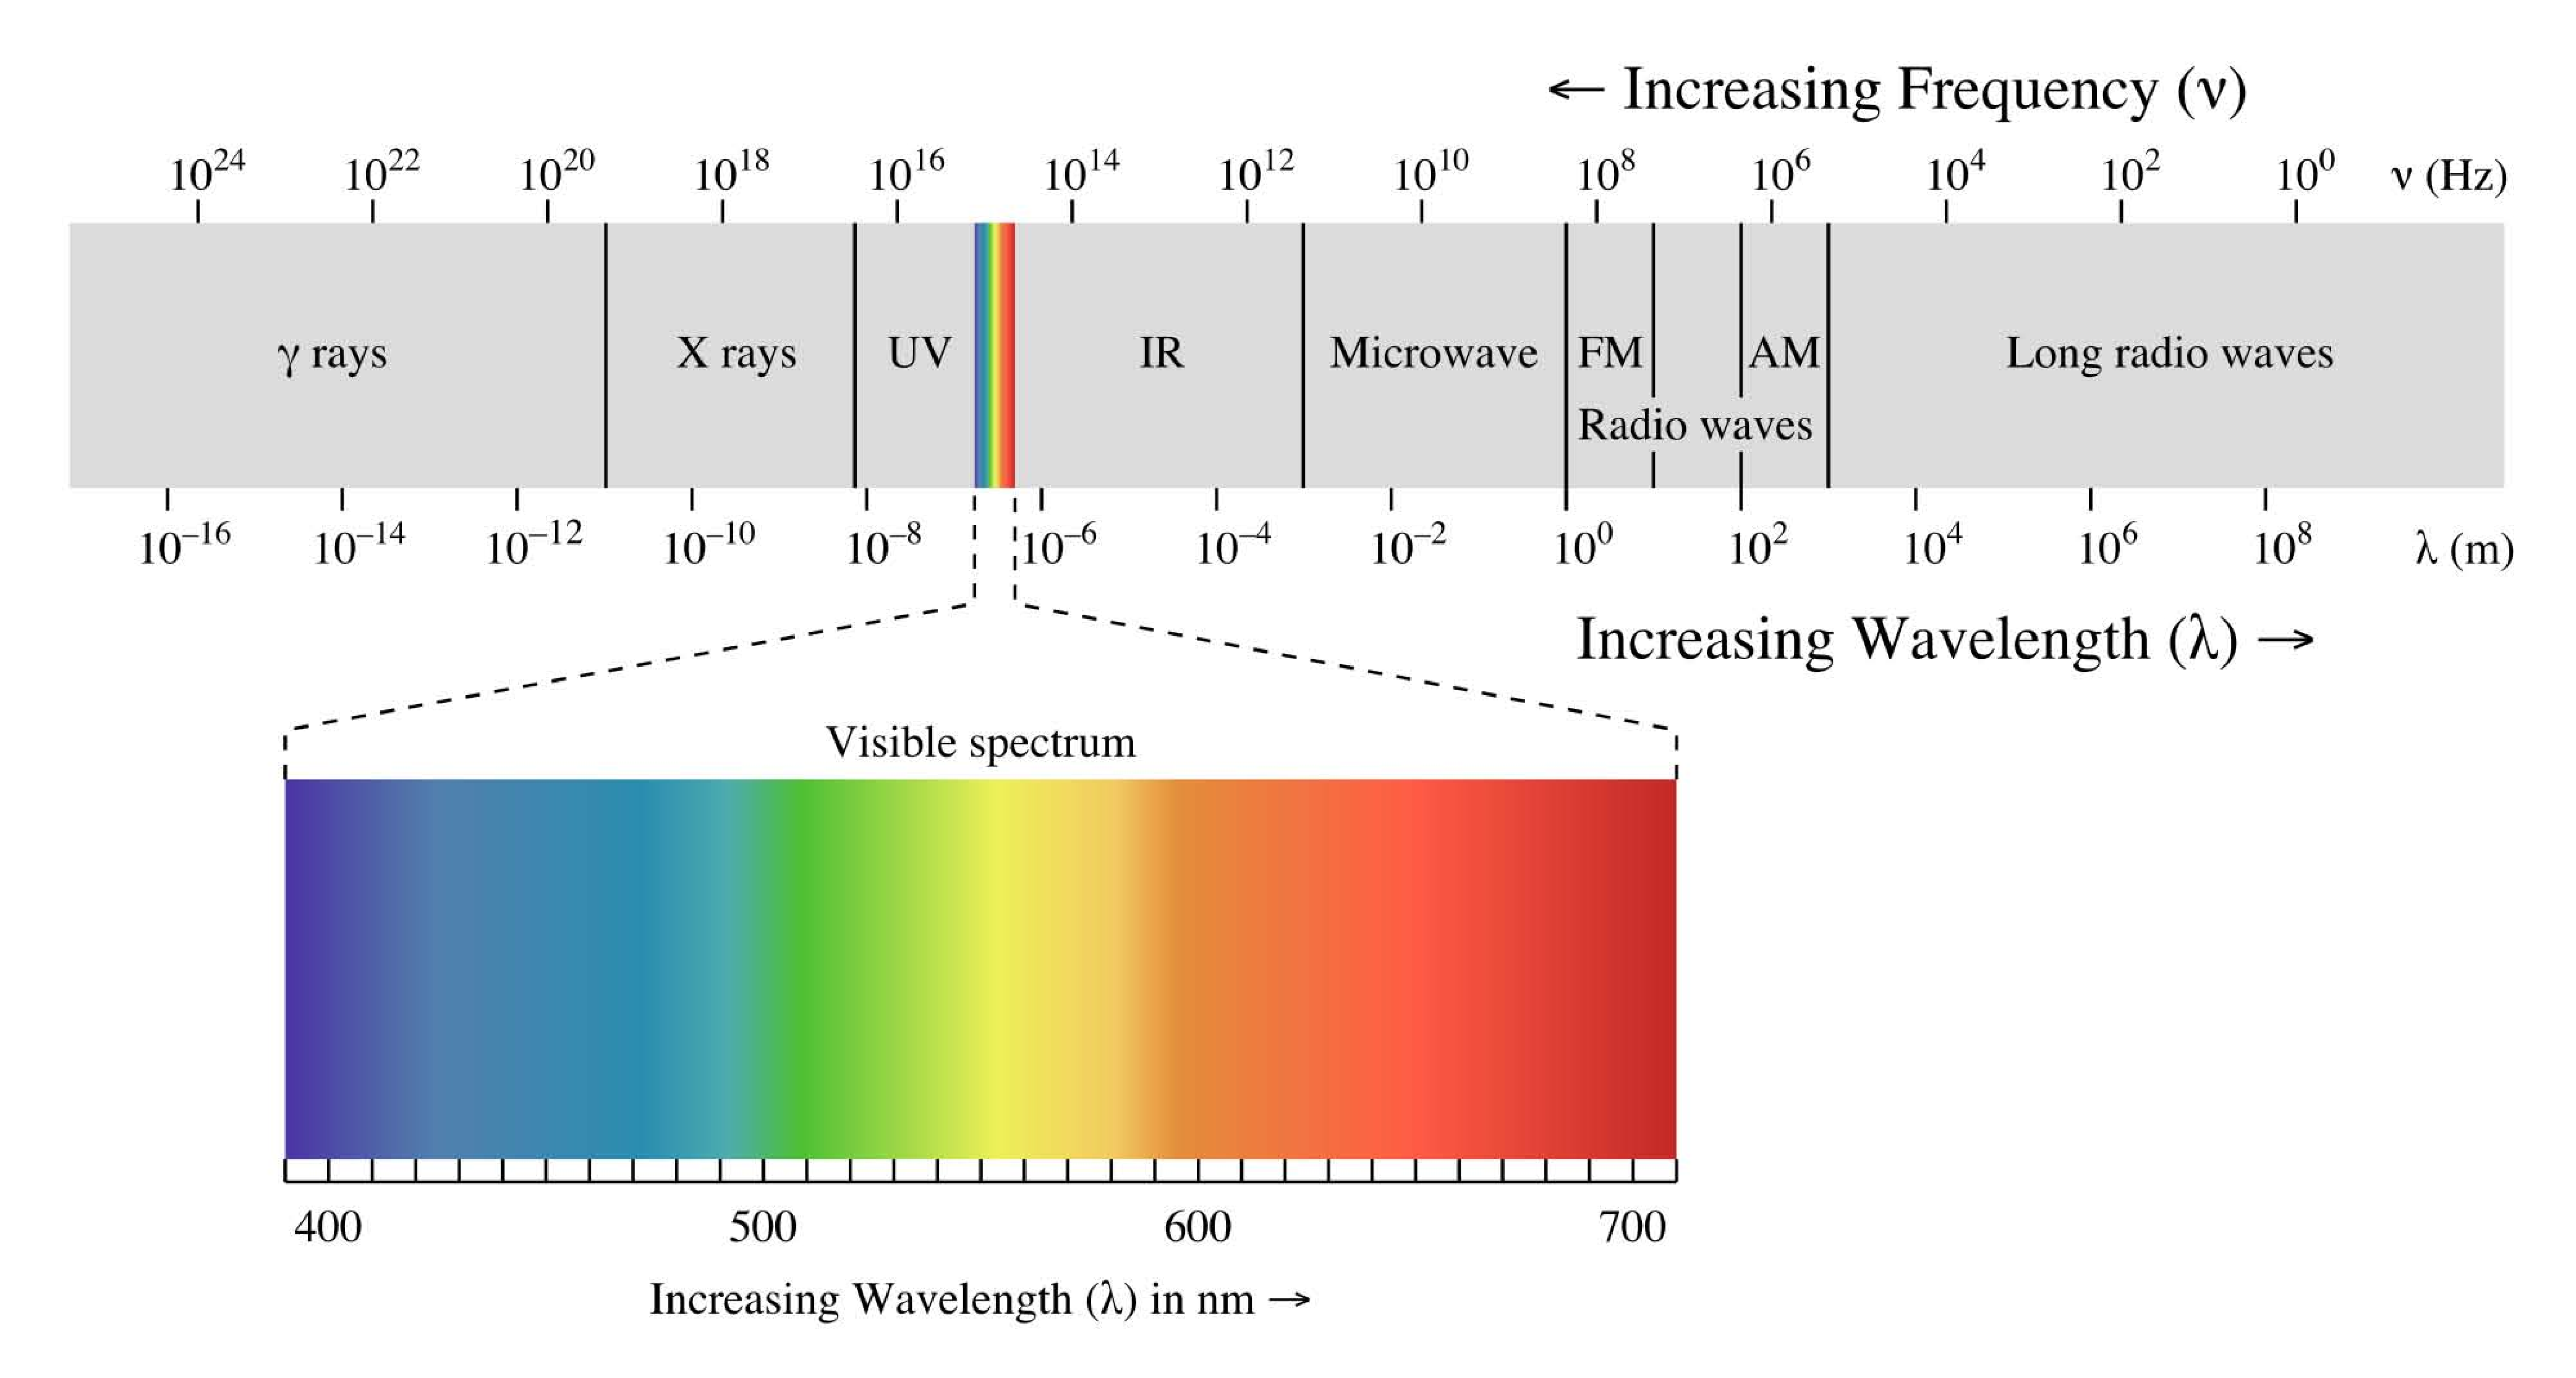
\includegraphics[width=11cm]{ch1/em_spectrum} % ͼƬ�������Դ�Щ��ĸ��ͷ
  \end{center}
\end{figure}

\end{frame}

%%%%%%%%%%%%%%%%%%%%%%%%%%%%%%%%%%%%%%%%%%%%%%%%%%%%%%%%%%%%%%%%%

\begin{frame}
\frametitle{\textsc{Electromagnetic Spectrum}}\transwipe % ͿĨЧ��
\vspace{-0.5cm}

{\scriptsize
\begin{table}[!h]
\rowcolors{1}{blue!20}{blue!10} \arrayrulecolor{blue!5}
\tabcolsep 2pt % ��
\renewcommand\arraystretch{1.1} % ��

\caption{ITU frequency band}\label{tab:frequency_band}
\vspace*{-15pt}
\begin{center}
%    \setlength{\extrarowheight}{2ex} % ÿ�и߶�
    \setlength{\arrayrulewidth}{1.3pt}
    \begin{tabular}{c|c|c|p{4.5cm}<{\centering} }
        \arrayrulecolor{black}\hline
        \rowcolor{blue!50}  Band name & Frequency & Wavelength in air & Example uses  \\   \hline
        ELF & 3-30Hz & 100,000km-10,000km & Submarine communication  \\
        SLF & 30-300Hz & 10,000km-1000km & Submarine communication  \\
        ULF & 300-3000Hz & 1000km-100km & Communication within mines  \\
        VLF & 3-30Hz & 100km-10km & Navigation, Geophysics  \\
        LF & 30-300kHz & 10km-1km & Navigation, Amateur radio, RFID, AM long-wave broadcasting  \\
        MF & 300-3000kHz & 1000m-100m & AM medium-wave broadcasts \\
        HF & 3-30MHz & 100m-10m & Shortwave broadcasts, RFID, Over-the-horizon radar \\
        VHF & 30-300MHz & 10m-1m & FM,TV,weather radio, Maritime Mobile communications  \\
        UHF & 300-3000MHz & 1m-100mm & TV, mobile phones, wireless LAN, Bluetooth, GPS, microwave ovens \\
        SHF & 3-30GHz & 100mm-10mm & radio astronomy, radars, satellites  \\
        EHF & 30-300GHz & 10mm-1mm & remote sensing, energy weapon  \\
        THF or THz & 300-3000GHz & 1mm-100$\mu$m & Terahertz imaging,Terahertz computing/communications  \\
        \hline
       \end{tabular}
\end{center}
\end{table}
}
\end{frame}

%%%%%%%%%%%%%%%%%%%%%%%%%%%%%%%%%%%%%%%%%%%%%%%%%%%%%%%%%%%%%%%%%

\begin{frame}%[shrink] % shrink��ЧʱhyperlinkʧЧ
\frametitle{\textsc{Radio Frequency Band}} \transsplithorizontalout% ˮƽ˺��(����)
\vspace{-0.55cm}
\begin{multicols}{2}
{\footnotesize
\begin{table}[!h]
\rowcolors{1}{blue!20}{blue!10} \arrayrulecolor{blue!5}
\tabcolsep 4pt % ��
\renewcommand\arraystretch{1.1} % ��
\caption{IEEE bands}\label{tab:IEEE_band} \vspace*{-5.8pt}
  \begin{center}
    \setlength{\arrayrulewidth}{1.3pt}
    \resizebox{4.7cm}{!}{
    \begin{tabular}{c|c}%{\temptablewidth}{@{\extracolsep{\fill}}|c|c|c|c|c|}
        \arrayrulecolor{black}\hline
        \rowcolor{blue!50} Band & Frequency range \\   \hline
        HF band & 3-30MHz \\
        VHF band & 30-300MHz\\
        UHF band & 300-3000MHz\\
        L band & 1-2GHz \\
        S band & 2-4GHz \\
        C band & 4-8GHz \\
        X band & 8-12GHz \\
        K{\tiny u} band & 12-18GHz \\
        K band & 18-27GHz \\
        K{\tiny a} band & 27-40GHz \\
        V band & 40-75GHz \\
        W band & 75-110GHz \\
        mm band & 110-300GHz \\
        \hline
    \end{tabular} }
  \end{center}
\end{table}

\begin{table}[!h]
\rowcolors{1}{blue!20}{blue!10} \arrayrulecolor{blue!5}
\tabcolsep 4pt % ��
\renewcommand\arraystretch{1.1} % ��
\caption{EU, NATO, US ECM}\label{tab:EU_band} \vspace*{-7pt}
  \begin{center}
    \setlength{\arrayrulewidth}{1.3pt}
    \resizebox{4.3cm}{!}{
    \begin{tabular}{c|c}%{\temptablewidth}{@{\extracolsep{\fill}}|c|c|c|c|c|}
        \arrayrulecolor{black}\hline
        \rowcolor{blue!50} Band & Frequency range  \\   \hline
        A band & 0-0.25GHz \\
        B band & 0.25-0.5GHz\\
        C band & 0.5-1.0GHz\\
        D band & 1-2GHz \\
        E band & 2-3GHz \\
        F band & 3-4GHz \\
        G band & 4-6GHz \\
        H band & 6-8GHz \\
        I band & 8-10GHz \\
        J band & 10-20GHz \\
        K band & 20-40GHz \\
        L band & 40-60GHz \\
        M band & 60-100GHz \\
        \hline
    \end{tabular} }
  \end{center}
\end{table}
}
\vspace{-0.5cm}\rightline{\hyperlink{sec:1}{\beamerreturnbutton{back}}}
\end{multicols}

%\vspace{-0.5cm}\rightline{\hyperlink{sec:1}{\beamerreturnbutton{back}}}
\end{frame}

%%%%%%%%%%%%%%%%%%%%%%%%%%%%%%%%%%%%%%%%%%%%%%%%%%%%%%%%%%%%%%%%%

%%%%%%%%%%%%%%%%%%%%%%%%%%%%%%%%%%%%%%%%%%%%%%%%%%%%%%%%%%%%%%%%%

\section[Antenna Basic ���߻���]{Antenna Basic} %[���У������]

%%%%%%%%%%%%%%%%%%%%%%%%%%%%%% ����Ŀ¼ҳ %%%%%%%%%%%%%%%%%%%%%%%%%%%%%%%%%%%

\begin{frame}%<beamer>
    \frametitle{\textsc{Contents}} \vspace{-0.85cm}\label{sec:2}
    \begin{multicols}{2}
    \begin{minipage}[t]{0.55\textwidth}
    \tableofcontents[currentsection,hideallsubsections]
    % [currentsection,hideallsubsections][sectionstyle=show/shaded,subsectionstyle=show/shaded/hide]
    \end{minipage}

    \begin{minipage}[t]{0.55\textwidth}
    \vspace{0.5cm}
    \begin{spacing}{0.9} % ������� ��Ҫ\usepackage{setspace}
    \begin{itemize}
        \item\hyperlink{subsec:2-1}{Definition of Antennas}
        \item\hyperlink{subsec:2-2}{Patterns}
        \item\hyperlink{subsec:2-3}{Beam Area}
        \item\hyperlink{subsec:2-4}{Directivity and Gain}
        \item\hyperlink{subsec:2-5}{Antenna Apertures}
        \item\hyperlink{subsec:2-6}{Radio Communication Link}
        \item\hyperlink{subsec:2-7}{Fields From Dipole}
        \item\hyperlink{subsec:2-8}{Antenna Field Zones}
        \item\hyperlink{subsec:2-9}{Shape-Impedance Considerations}
        \item\hyperlink{subsec:2-10}{Polarization}
    \end{itemize}
    \end{spacing}
    \end{minipage}
    \end{multicols}
\end{frame}

%%%%%%%%%%%%%%%%%%%%%%%%%%%%%%%%%%%%%%%%%%%%%%%%%%%%%%%%%%%%%%%%%
\subsection[Definition of Antennas ���ߵĶ���]{Definition of Antennas}\label{subsec:2-1}
%%%%%%%%%%%%%%%%%%%%%%%%%%%%%%%%%%%%%%%%%%%%%%%%%%%%%%%%%%%%%%%%%

\begin{frame}
\frametitle{\textsc{What is Antenna?}} \transblindshorizontal % ˮƽ����Ч��
\begin{multicols}{3}
\begin{figure}
  \begin{center}
    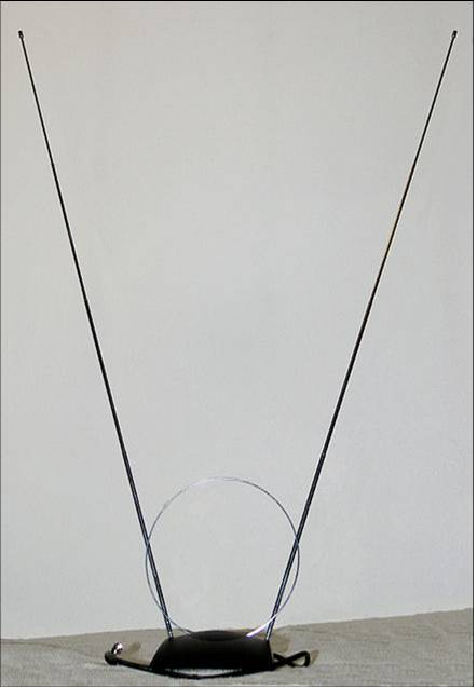
\includegraphics[width=3cm]{ch2/antenna1} % ͼƬ�������Դ�Щ��ĸ��ͷ
  \end{center}
\end{figure}
\begin{figure}
  \begin{center}
    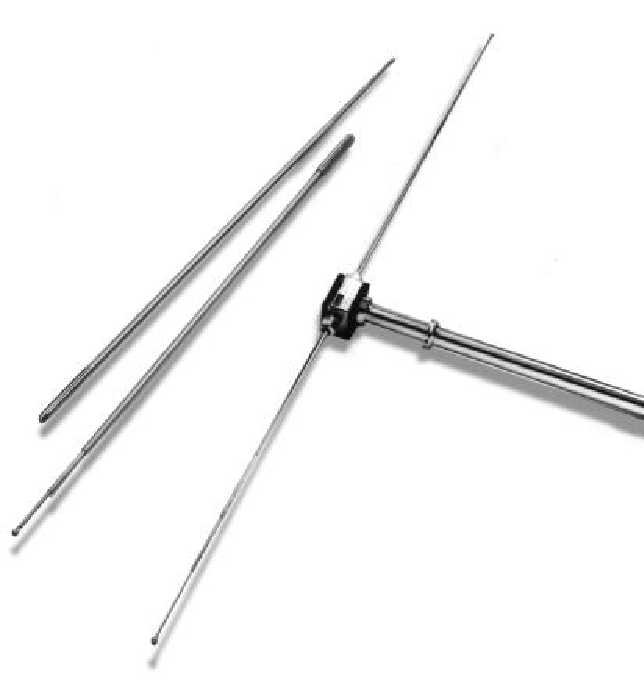
\includegraphics[width=3cm]{ch2/antenna2} % ͼƬ�������Դ�Щ��ĸ��ͷ
  \end{center}
\end{figure}
\begin{figure}
  \begin{center}
    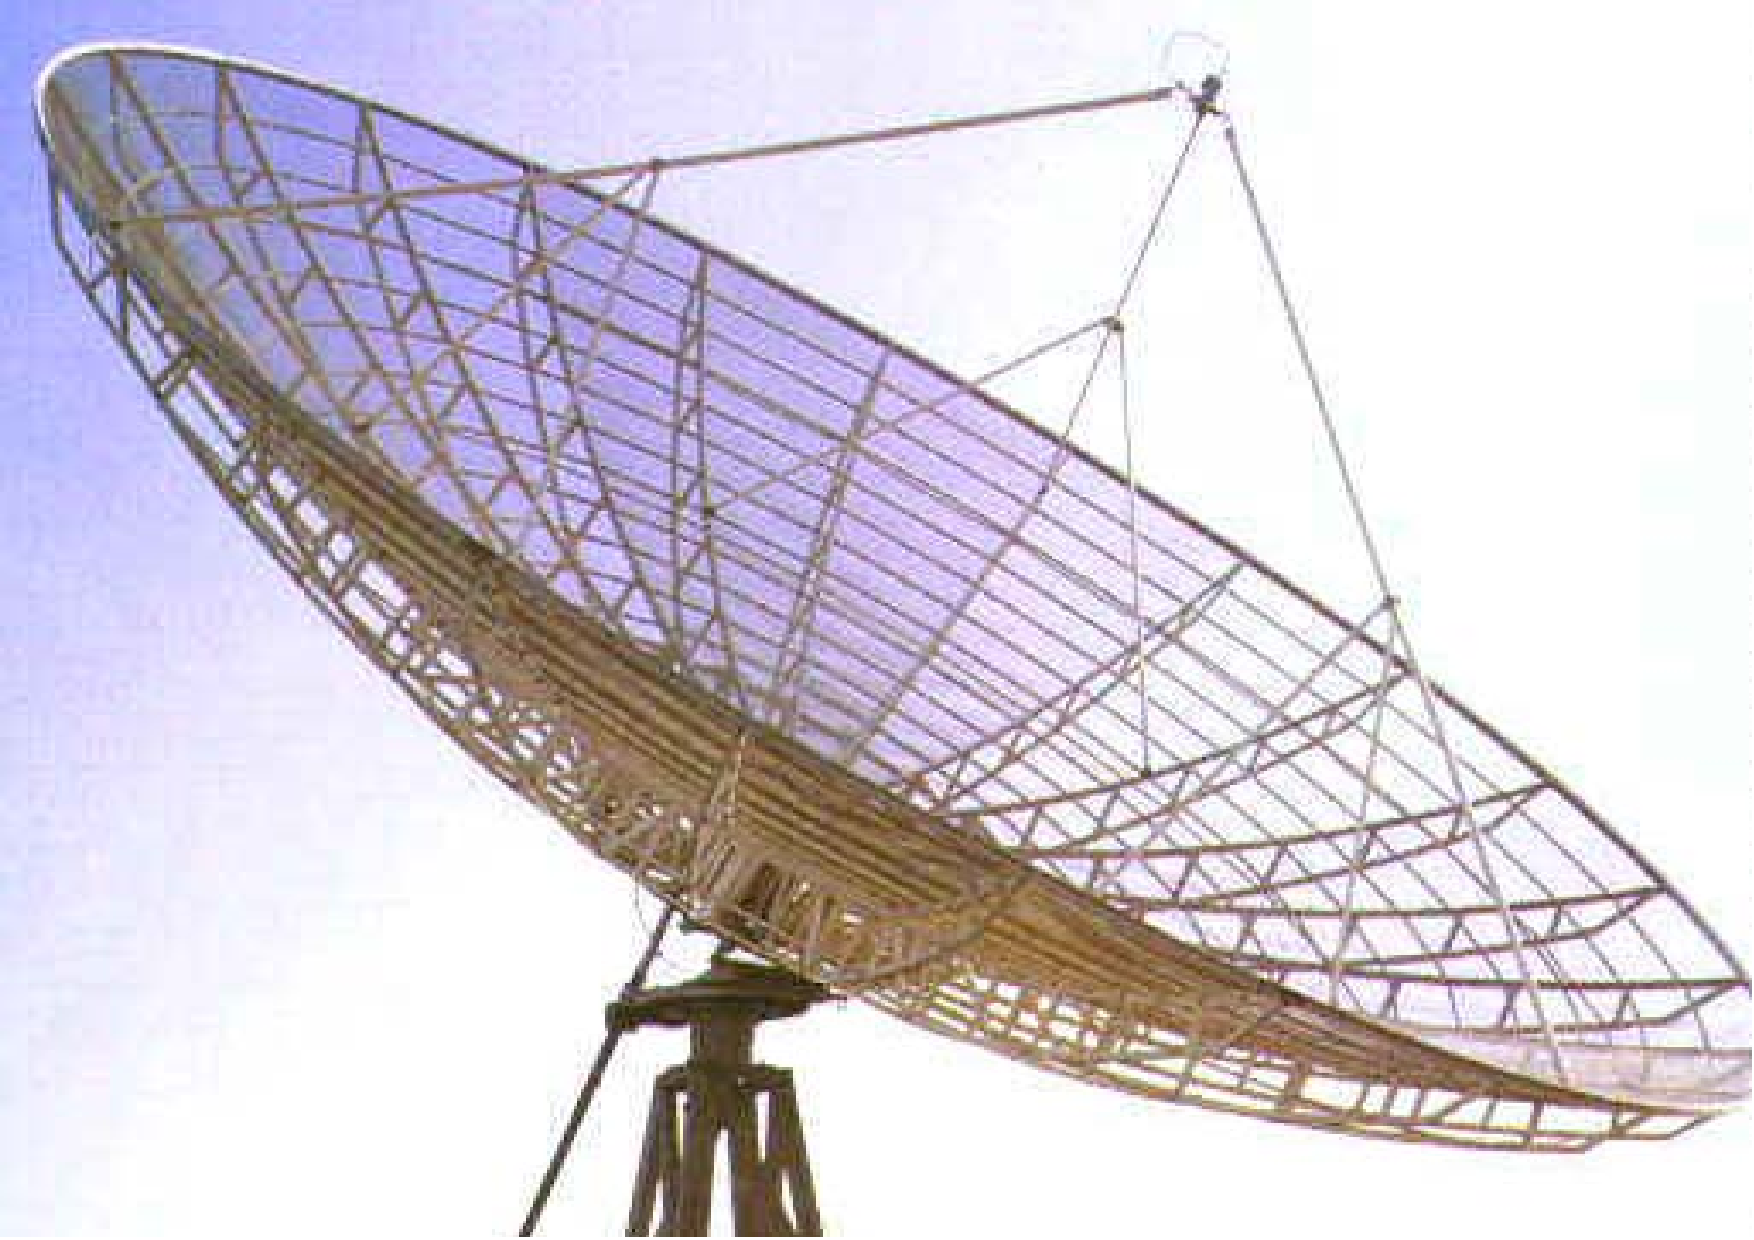
\includegraphics[width=3cm]{ch2/antenna3} % ͼƬ�������Դ�Щ��ĸ��ͷ
  \end{center}
\end{figure}
\begin{figure}
  \begin{center}
    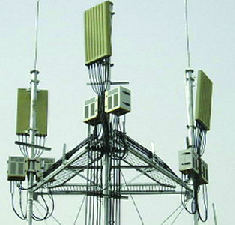
\includegraphics[width=3cm]{ch2/antenna4} % ͼƬ�������Դ�Щ��ĸ��ͷ
  \end{center}
\end{figure}
\begin{figure}
  \begin{center}
    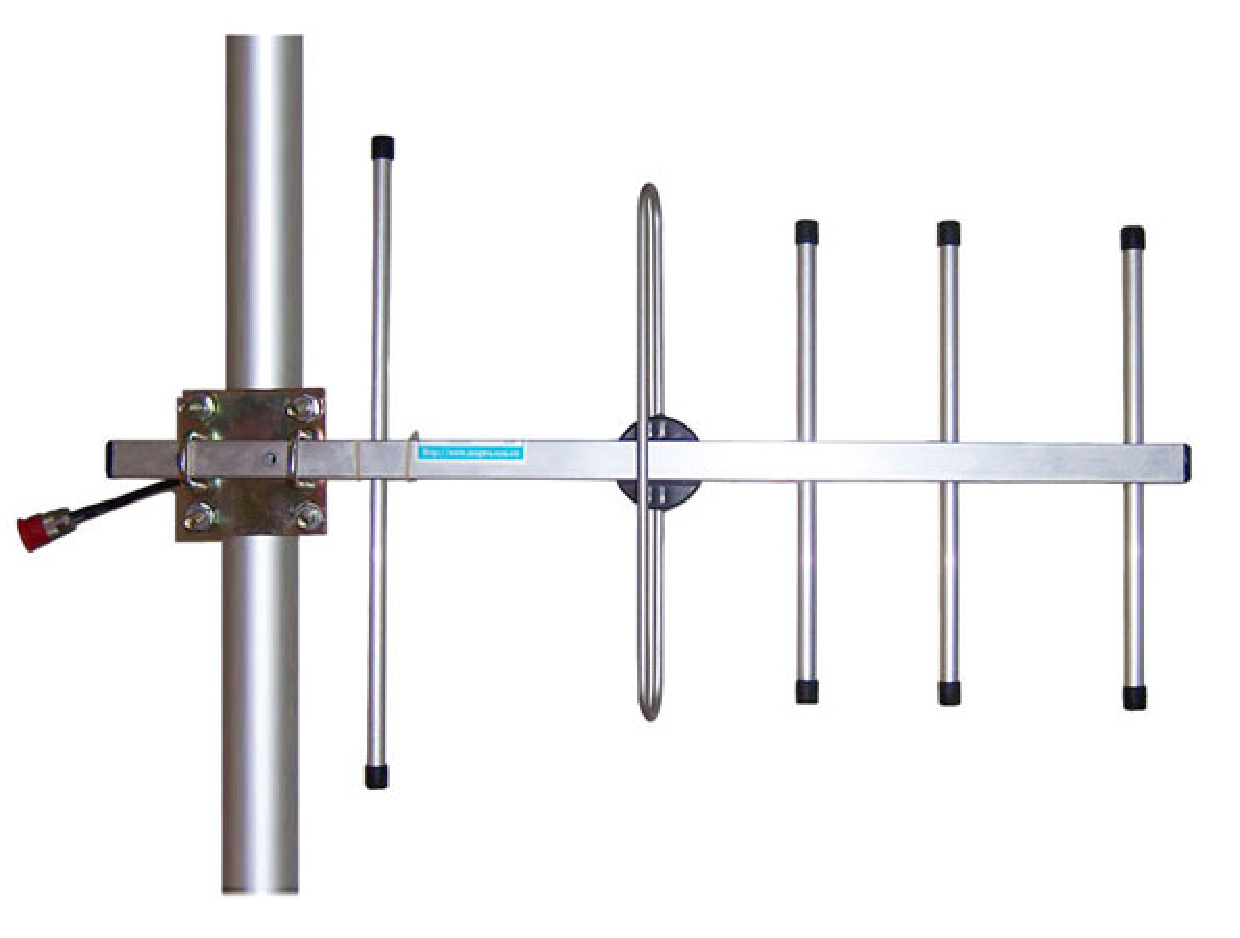
\includegraphics[width=3cm]{ch2/antenna5} % ͼƬ�������Դ�Щ��ĸ��ͷ
  \end{center}
\end{figure}

\end{multicols}
\end{frame}

%%%%%%%%%%%%%%%%%%%%%%%%%%%%%%%%%%%%%%%%%%%%%%%%%%%%%%%%%%%%%%%%%

\begin{frame}
\frametitle{\textsc{What is Antenna?}}
\begin{multicols}{3}
\transblindsvertical %  ��ֱ����Ч��
\begin{figure}
  \begin{center}
    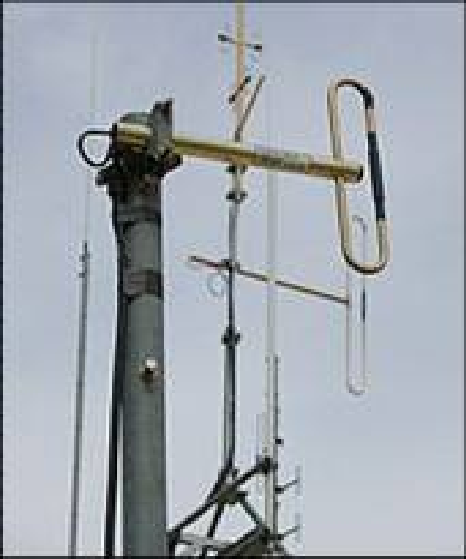
\includegraphics[width=3cm]{ch2/antenna6} % ͼƬ�������Դ�Щ��ĸ��ͷ
  \end{center}
\end{figure}
\begin{figure}
  \begin{center}
    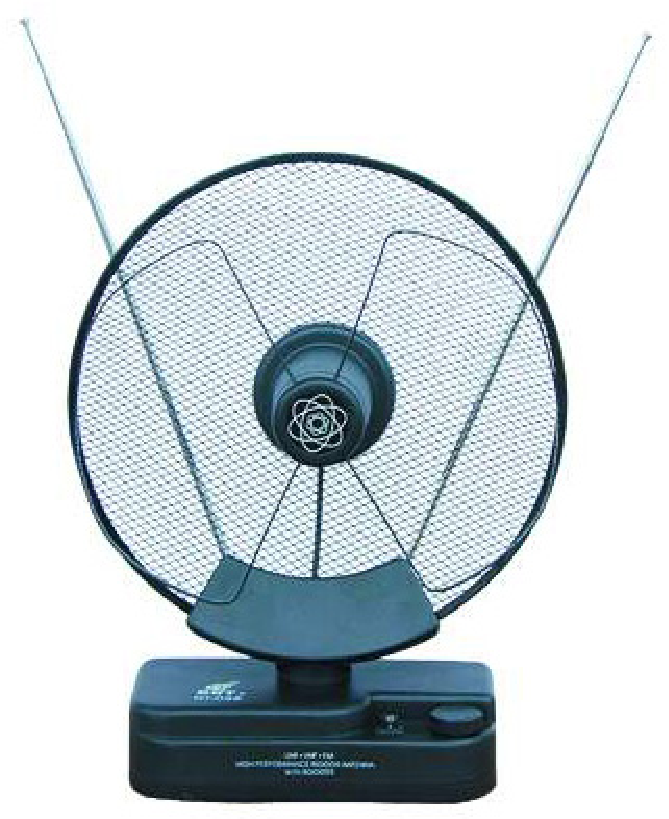
\includegraphics[width=3cm]{ch2/antenna7} % ͼƬ�������Դ�Щ��ĸ��ͷ
  \end{center}
\end{figure}
\begin{figure}
  \begin{center}
    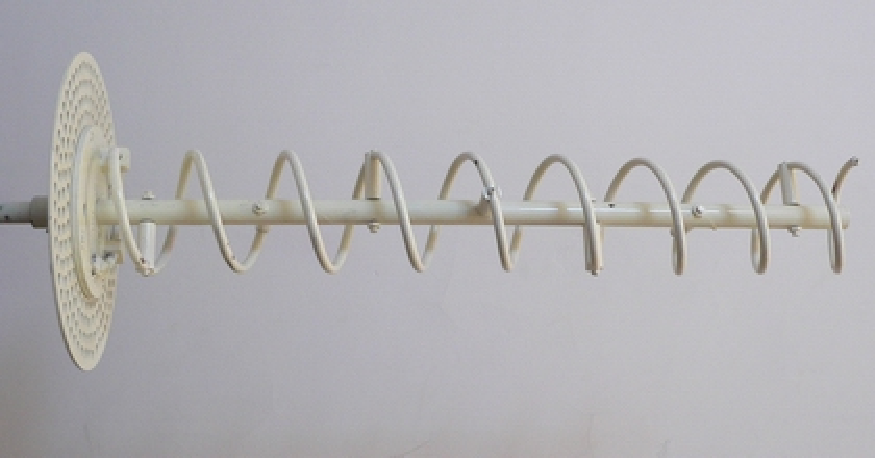
\includegraphics[width=3cm]{ch2/antenna8} % ͼƬ�������Դ�Щ��ĸ��ͷ
  \end{center}
\end{figure}
\begin{figure}
  \begin{center}
    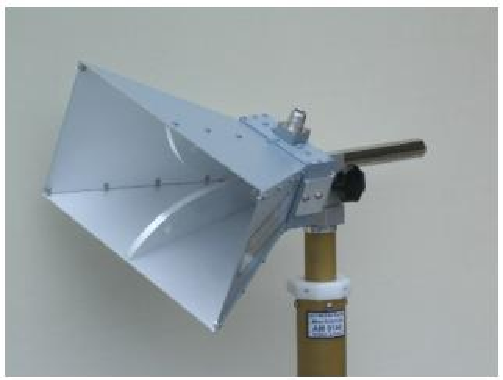
\includegraphics[width=3cm]{ch2/antenna9} % ͼƬ�������Դ�Щ��ĸ��ͷ
  \end{center}
\end{figure}
\begin{figure}
  \begin{center}
    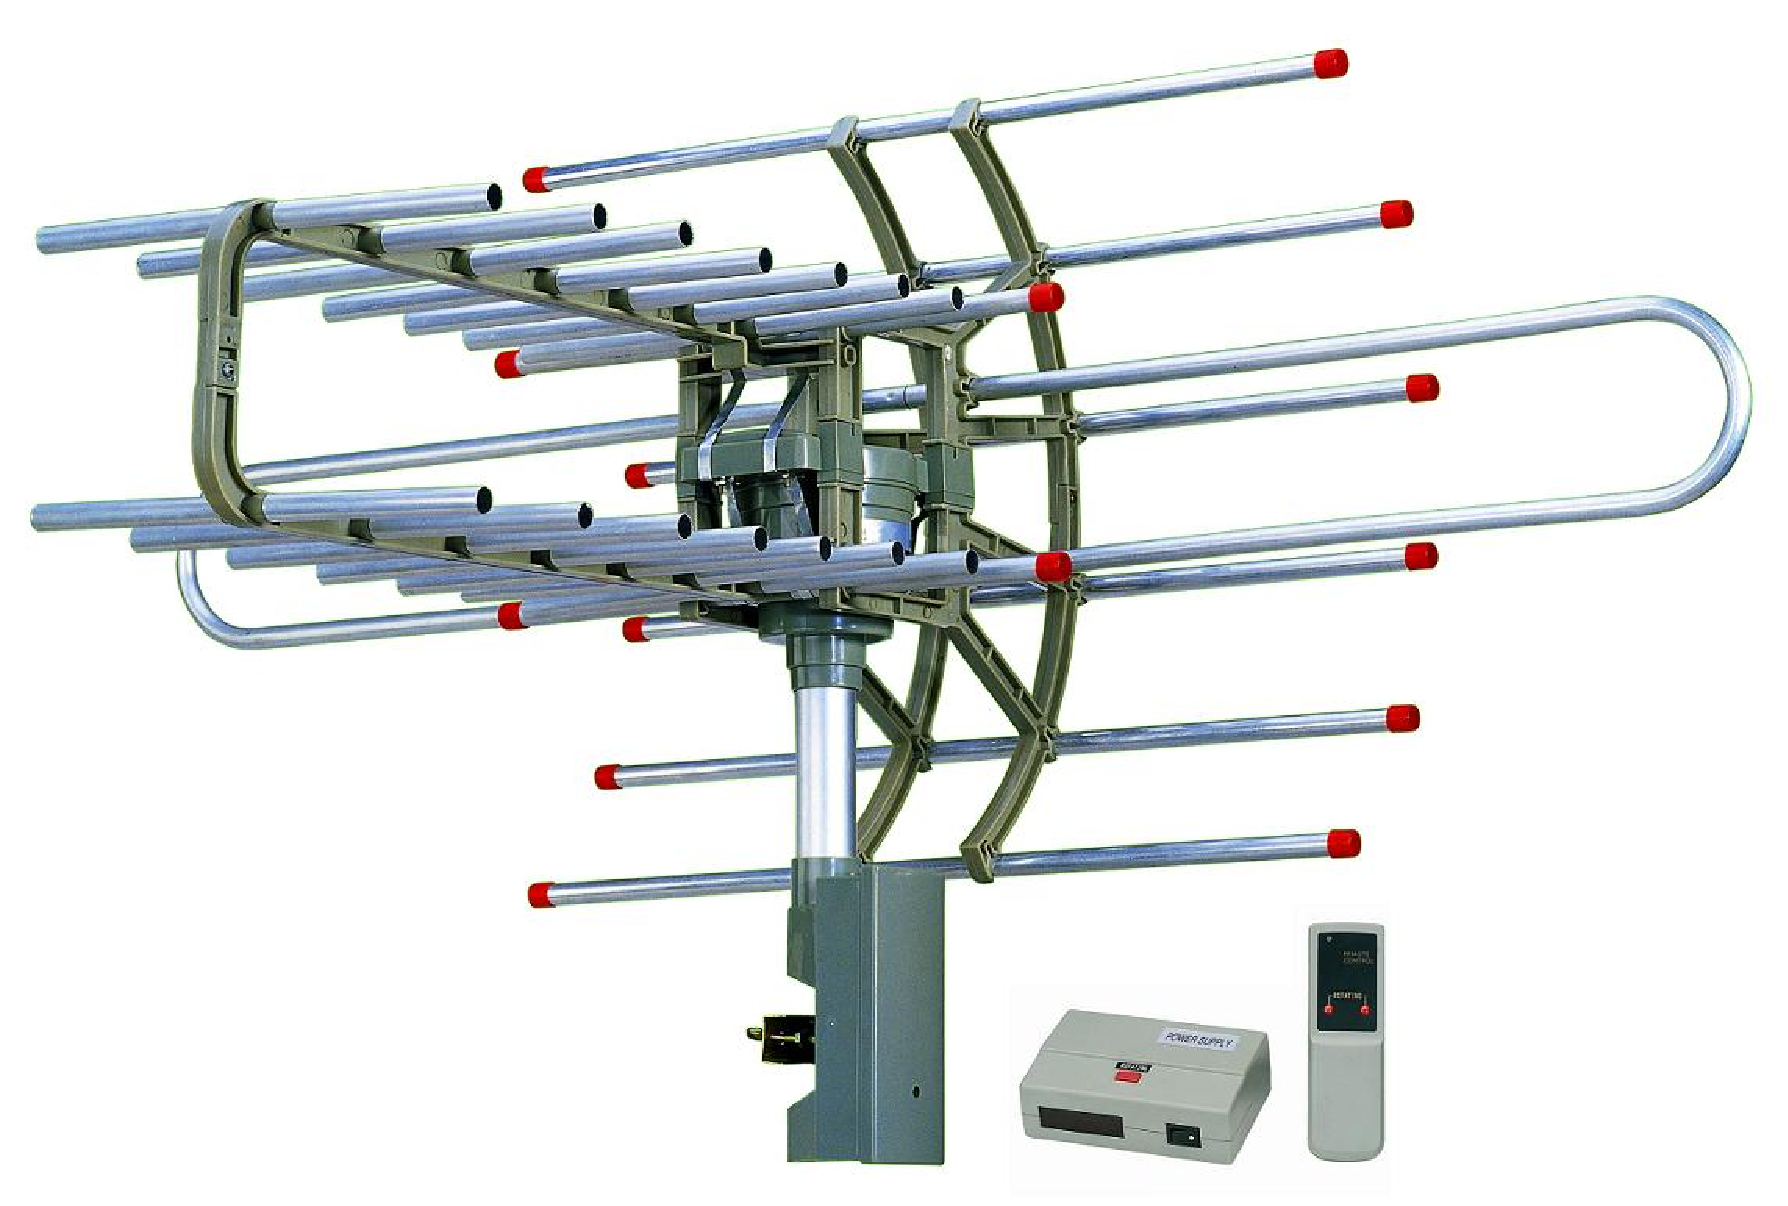
\includegraphics[width=3cm]{ch2/antenna10} % ͼƬ�������Դ�Щ��ĸ��ͷ
  \end{center}
\end{figure}

\end{multicols}
\end{frame}

%%%%%%%%%%%%%%%%%%%%%%%%%%%%%%%%%%%%%%%%%%%%%%%%%%%%%%%%%%%%%%%%%
\begin{frame}
\frametitle{\textsc{What is Antenna?}}
\begin{multicols}{3}
\transboxout  %  ���Ľǵ�����
\begin{figure}
  \begin{center}
    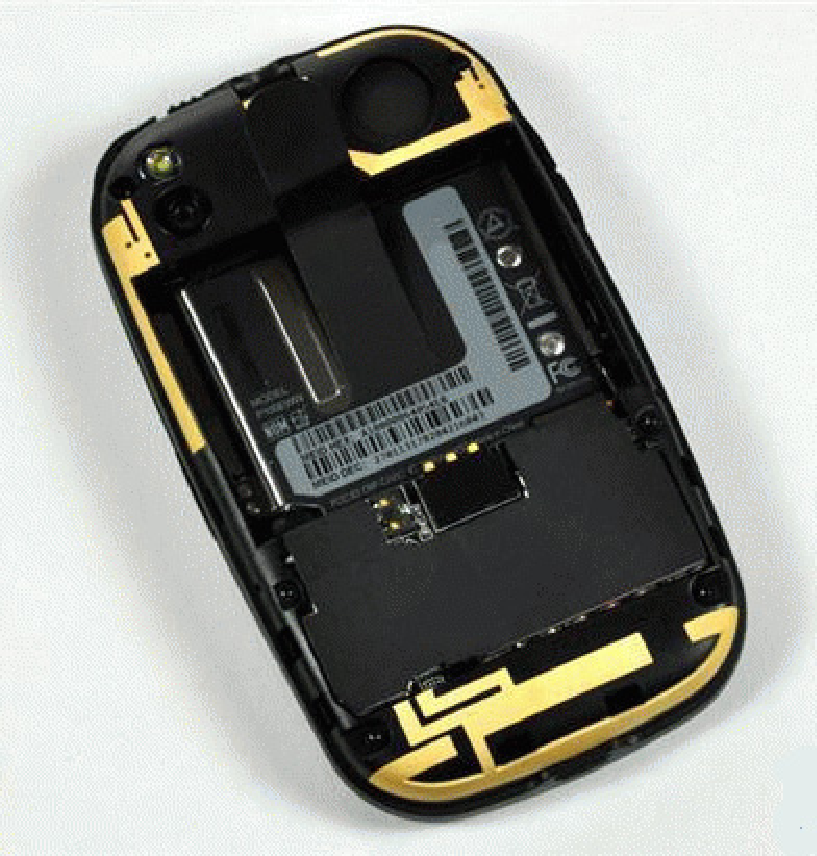
\includegraphics[width=3cm]{ch2/antenna11} % ͼƬ�������Դ�Щ��ĸ��ͷ
  \end{center}
\end{figure}
\begin{figure}
  \begin{center}
    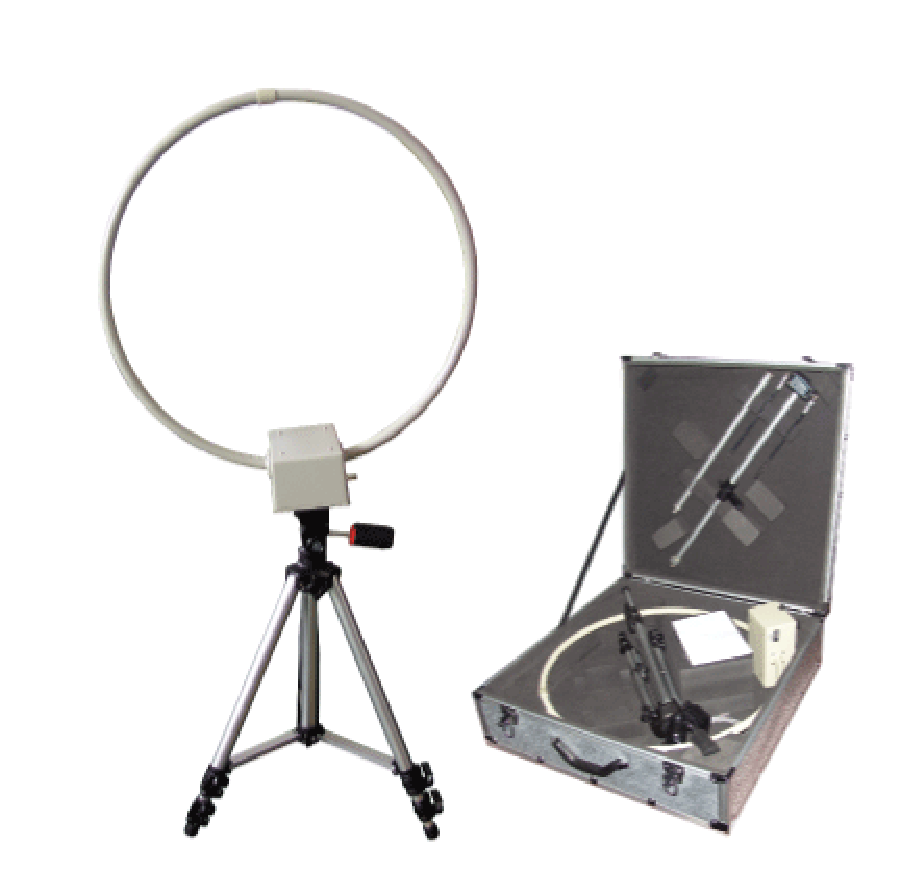
\includegraphics[width=3cm]{ch2/antenna12} % ͼƬ�������Դ�Щ��ĸ��ͷ
  \end{center}
\end{figure}
\begin{figure}
  \begin{center}
    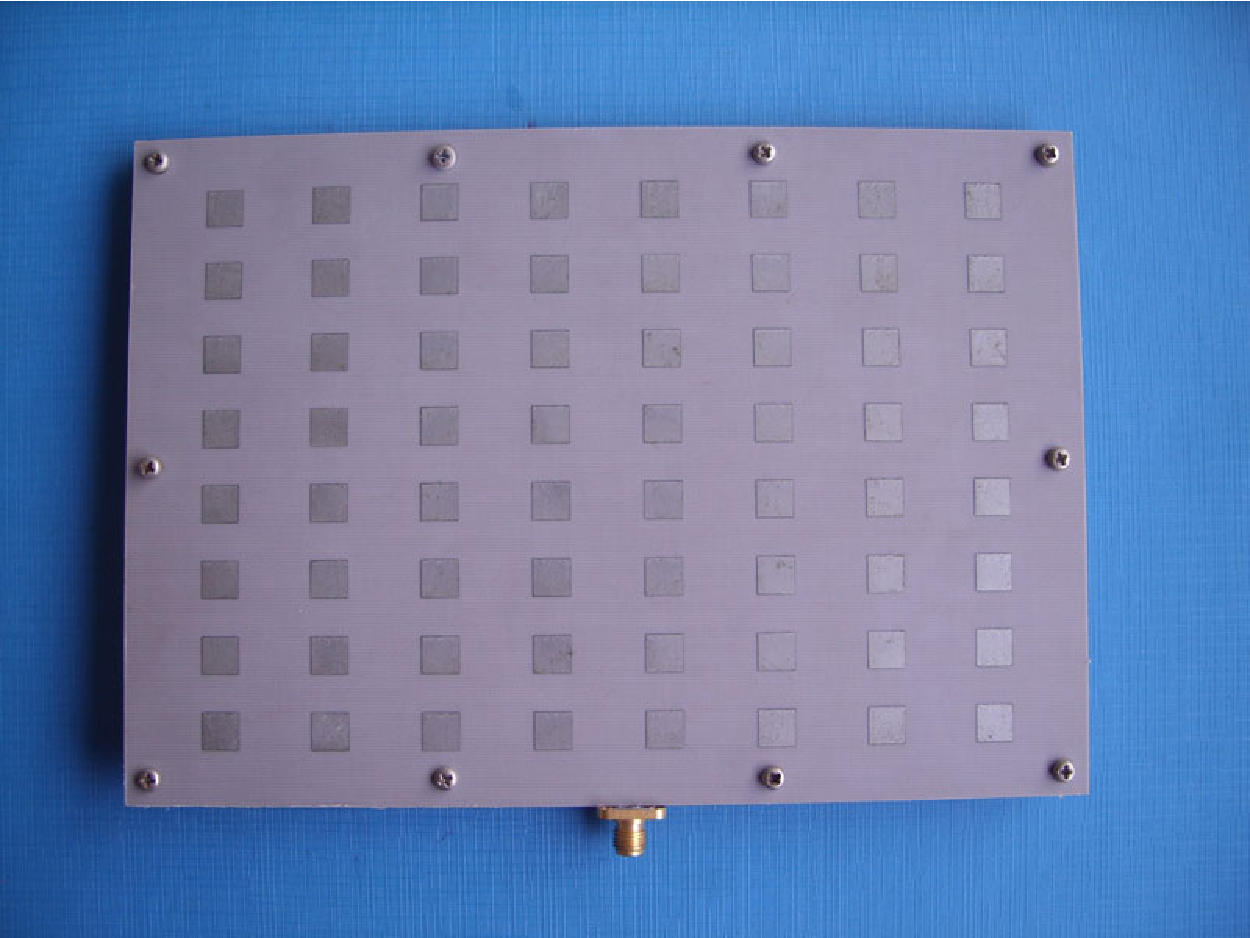
\includegraphics[width=3cm]{ch2/antenna13} % ͼƬ�������Դ�Щ��ĸ��ͷ
  \end{center}
\end{figure}

\end{multicols}
\end{frame}

%%%%%%%%%%%%%%%%%%%%%%%%%%%%%%%%%%%%%%%%%%%%%%%%%%%%%%%%%%%%%%%%%

\begin{frame}% [shrink]
\frametitle{\textsc{Definition of Antenna}}%\transwipe % ͿĨЧ��

\hilite<1>Regardless of antenna type, all involve the same basic
principle that radiation is produced by accelerated charge.
���ۺ������ͣ����߶��ǻ��ڼ��ٵ�ɲ�������Ĺ�ͬԭ����\pause

\hilite<2>The {\bf basic equation of radiation} may be expressed
simply as
\begin{equation}\label{eq:radiation}
    \dot{I}L = Q\dot{v}
\end{equation}
\vspace{-0.1cm} where
\begin{eqnarray*}
% \nonumber to remove numbering (before each equation)
  \dot{I} \!\!&=&\!\! \text{time-changing current}, \rm A/s \\
  L \!\!&=&\!\! \text{length of current element}, \rm m \\
  Q \!\!&=&\!\! \text{charge}, \mathrm{C} \\
  \dot{v} \!\!&=&\!\! \text{time change of velocity}, \rm m/s^2
\end{eqnarray*}

\end{frame}

%%%%%%%%%%%%%%%%%%%%%%%%%%%%%%%%%%%%%%%%%%%%%%%%%%%%%%%%%%%%%%%%%

\begin{frame}
\frametitle{\textsc{Definition of Antenna}}\transsplithorizontalout %  ˮƽ˺��(����)

\begin{figure}
  \begin{center}
    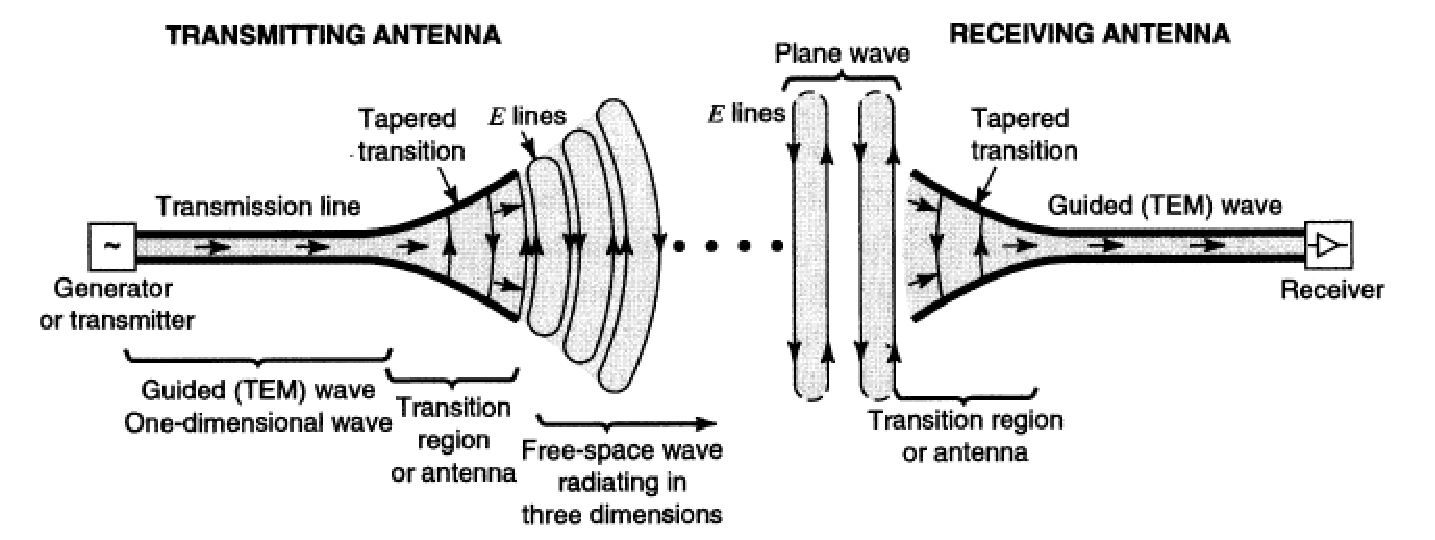
\includegraphics[width=11cm]{ch2/antenna_region} % ͼƬ�������Դ�Щ��ĸ��ͷ
  \end{center}
\end{figure}

\end{frame}

%%%%%%%%%%%%%%%%%%%%%%%%%%%%%%%%%%%%%%%%%%%%%%%%%%%%%%%%%%%%%%%%%

\begin{frame}
\frametitle{\textsc{Definition of Antenna}}

\begin{itemize}
\hilite<1>\item An antenna, also known as an aerial, a transducer
designed to transmit or receive electromagnetic waves.
�����Ƿ������յ�Ų��Ļ�������(Wikipedia)\pause

\hilite<2>\item An antenna, a means for radiating or receiving radio
waves. �����Ƿ������յ�Ų��ķ�����(IEEE Std 1974�C1983)\pause

\hilite<3>\item An antenna is a transition device, or transducer,
between a guided wave and a free-space wave, or vice-versa.
������һ�ֵ��в������ɿռ䲨֮���ת������������
\end{itemize}

\rightline{\hyperlink{sec:2}{\beamerreturnbutton{back}} }

\end{frame}

%%%%%%%%%%%%%%%%%%%%%%%%%%%%%%%%%%%%%%%%%%%%%%%%%%%%%%%%%%%%%%%%%
\subsection[Patterns ����ͼ]{Patterns}\label{subsec:2-2}
%%%%%%%%%%%%%%%%%%%%%%%%%%%%%%%%%%%%%%%%%%%%%%%%%%%%%%%%%%%%%%%%%

\begin{frame}
\frametitle{\textsc{Patterns}}

\end{frame}

%%%%%%%%%%%%%%%%%%%%%%%%%%%%%%%%%%%%%%%%%%%%%%%%%%%%%%%%%%%%%%%%%

\begin{frame}
\frametitle{\textsc{Radiation Intensity}}


\rightline{\hyperlink{sec:2}{\beamerreturnbutton{back}} }
\end{frame}

%%%%%%%%%%%%%%%%%%%%%%%%%%%%%%%%%%%%%%%%%%%%%%%%%%%%%%%%%%%%%%%%%
\subsection[Beam Area ������Χ]{Beam Area}\label{subsec:2-3}
%%%%%%%%%%%%%%%%%%%%%%%%%%%%%%%%%%%%%%%%%%%%%%%%%%%%%%%%%%%%%%%%%

\begin{frame}
\frametitle{\textsc{Beam Area}}


\end{frame}

%%%%%%%%%%%%%%%%%%%%%%%%%%%%%%%%%%%%%%%%%%%%%%%%%%%%%%%%%%%%%%%%%

\begin{frame}
\frametitle{\textsc{Beam Efficiency}}

\rightline{\hyperlink{sec:2}{\beamerreturnbutton{back}} }
\end{frame}

%%%%%%%%%%%%%%%%%%%%%%%%%%%%%%%%%%%%%%%%%%%%%%%%%%%%%%%%%%%%%%%%%
\subsection[Directivity and Gain �����Ժ�����]{Directivity and Gain}\label{subsec:2-4}
%%%%%%%%%%%%%%%%%%%%%%%%%%%%%%%%%%%%%%%%%%%%%%%%%%%%%%%%%%%%%%%%%

\begin{frame}
\frametitle{\textsc{Directivity and Gain}}


\end{frame}

%%%%%%%%%%%%%%%%%%%%%%%%%%%%%%%%%%%%%%%%%%%%%%%%%%%%%%%%%%%%%%%%%

\begin{frame}
\frametitle{\textsc{Resolution}}

\rightline{\hyperlink{sec:2}{\beamerreturnbutton{back}} }
\end{frame}

%%%%%%%%%%%%%%%%%%%%%%%%%%%%%%%%%%%%%%%%%%%%%%%%%%%%%%%%%%%%%%%%%
\subsection[Antenna Apertures ���߿ھ�]{Antenna Apertures}\label{subsec:2-5}
%%%%%%%%%%%%%%%%%%%%%%%%%%%%%%%%%%%%%%%%%%%%%%%%%%%%%%%%%%%%%%%%%

\begin{frame}
\frametitle{\textsc{Antenna Apertures}}


\end{frame}

%%%%%%%%%%%%%%%%%%%%%%%%%%%%%%%%%%%%%%%%%%%%%%%%%%%%%%%%%%%%%%%%%

\begin{frame}
\frametitle{\textsc{Effective Height}}

\rightline{\hyperlink{sec:2}{\beamerreturnbutton{back}} }
\end{frame}

%%%%%%%%%%%%%%%%%%%%%%%%%%%%%%%%%%%%%%%%%%%%%%%%%%%%%%%%%%%%%%%%%
\subsection[Radio Communication Link ���ߵ�ͨ����·]{Radio Communication Link}\label{subsec:2-6}
%%%%%%%%%%%%%%%%%%%%%%%%%%%%%%%%%%%%%%%%%%%%%%%%%%%%%%%%%%%%%%%%%

\begin{frame}
\frametitle{\textsc{Radio Communication Link}} \

\rightline{\hyperlink{sec:2}{\beamerreturnbutton{back}} }
\end{frame}

%%%%%%%%%%%%%%%%%%%%%%%%%%%%%%%%%%%%%%%%%%%%%%%%%%%%%%%%%%%%%%%%%
\subsection[Fields From Oscillation Dipole ��ż���Ӳ����ij�]{Fields From Dipole}\label{subsec:2-7}
%%%%%%%%%%%%%%%%%%%%%%%%%%%%%%%%%%%%%%%%%%%%%%%%%%%%%%%%%%%%%%%%%

\begin{frame}
\frametitle{\textsc{Fields From Oscillation Dipole}}

\rightline{\hyperlink{sec:2}{\beamerreturnbutton{back}} }
\end{frame}

%%%%%%%%%%%%%%%%%%%%%%%%%%%%%%%%%%%%%%%%%%%%%%%%%%%%%%%%%%%%%%%%%
\subsection[Antenna Field Zones ���ߵij���]{Antenna Field Zones}\label{subsec:2-8}
%%%%%%%%%%%%%%%%%%%%%%%%%%%%%%%%%%%%%%%%%%%%%%%%%%%%%%%%%%%%%%%%%

\begin{frame}
\frametitle{\textsc{Antenna Field Zones}}

\rightline{\hyperlink{sec:2}{\beamerreturnbutton{back}} }
\end{frame}

%%%%%%%%%%%%%%%%%%%%%%%%%%%%%%%%%%%%%%%%%%%%%%%%%%%%%%%%%%%%%%%%%
\subsection[Shape-Impedance Considerations ��״-�迹������]{Shape-Impedance Considerations}\label{subsec:2-9}
%%%%%%%%%%%%%%%%%%%%%%%%%%%%%%%%%%%%%%%%%%%%%%%%%%%%%%%%%%%%%%%%%

\begin{frame}
\frametitle{\textsc{Shape-Impedance Considerations}}

\rightline{\hyperlink{sec:2}{\beamerreturnbutton{back}} }
\end{frame}

%%%%%%%%%%%%%%%%%%%%%%%%%%%%%%%%%%%%%%%%%%%%%%%%%%%%%%%%%%%%%%%%%
\subsection[Polarization ����]{Polarization}\label{subsec:2-10}
%%%%%%%%%%%%%%%%%%%%%%%%%%%%%%%%%%%%%%%%%%%%%%%%%%%%%%%%%%%%%%%%%

\begin{frame}
\frametitle{\textsc{Polarization}}


\end{frame}

%%%%%%%%%%%%%%%%%%%%%%%%%%%%%%%%%%%%%%%%%%%%%%%%%%%%%%%%%%%%%%%%%

\begin{frame}
\frametitle{\textsc{Poynting Vector}}


\end{frame}

%%%%%%%%%%%%%%%%%%%%%%%%%%%%%%%%%%%%%%%%%%%%%%%%%%%%%%%%%%%%%%%%%

\begin{frame}
\frametitle{\textsc{Poincar\'{e} Sphere}} 

\rightline{\hyperlink{sec:2}{\beamerreturnbutton{back}} }
\end{frame}

%%%%%%%%%%%%%%%%%%%%%%%%%%%%%%%%%%%%%%%%%%%%%%%%%%%%%%%%%%%%%%%%%

%%%%%%%%%%%%%%%%%%%%%%%%%%%%%%%%%%%%%%%%%%%%%%%%%%%%%%%%%%%%%%%%%

\section[The Antenna Family ���߼���]{The Antenna Family}

%%%%%%%%%%%%%%%%%%%%%%%%%%%%%% ����Ŀ¼ҳ %%%%%%%%%%%%%%%%%%%%%%%%%%%%%%%%%%%

\begin{frame}%<beamer>
    \frametitle{\textsc{Contents}} \vspace{-0.85cm}\label{sec:3}
    \begin{multicols}{2}
    \begin{minipage}[t]{0.55\textwidth}
    \tableofcontents[currentsection,hideallsubsections]
    % [currentsection,hideallsubsections][sectionstyle=show/shaded,subsectionstyle=show/shaded/hide]
    \end{minipage}

    \begin{minipage}[t]{0.55\textwidth}
    \vspace{0.6cm}
    \begin{spacing}{0.9} % ������� ��Ҫ\usepackage{setspace}
    \begin{itemize}
        \item\hyperlink{subsec:3-1}{Loops, Dipole and Slots}
        \item\hyperlink{subsec:3-2}{Coaxial-Line Antennas}
        \item\hyperlink{subsec:3-3}{Twin-Line Antennas}
        \item\hyperlink{subsec:3-4}{Waveguide Antennas}
        \item\hyperlink{subsec:3-5}{Flat-Sheet Reflector Antennas}
        \item\hyperlink{subsec:3-6}{Radio Communication Link}
        \item\hyperlink{subsec:3-7}{Fields From Dipole}
        \item\hyperlink{subsec:3-8}{Antenna Field Zones}
        \item\hyperlink{subsec:3-9}{Shape-Impedance Considerations}
    \end{itemize}
    \end{spacing}
    \end{minipage}
    \end{multicols}
\end{frame}

%%%%%%%%%%%%%%%%%%%%%%%%%%%%%%%%%%%%%%%%%%%%%%%%%%%%%%%%%%%%%%%%%
\subsection[Loops, Dipole and Slots ���Ρ�ż���Ӻͷ�϶����]{Loops, Dipole and Slots}\label{subsec:3-1}
%%%%%%%%%%%%%%%%%%%%%%%%%%%%%%%%%%%%%%%%%%%%%%%%%%%%%%%%%%%%%%%%%

\begin{frame}
\frametitle{\textsc{Loops, Dipole and Slots}}

\end{frame}


%%%%%%%%%%%%%%%%%%%%%%%%%%%%%%%%%%%%%%%%%%%%%%%%%%%%%%%%%%%%%%%%%
\subsection[Opened-Out Coaxial-Line Antennas �ſ���ͬ��������]{Coaxial-Line Antennas}\label{subsec:3-2}
%%%%%%%%%%%%%%%%%%%%%%%%%%%%%%%%%%%%%%%%%%%%%%%%%%%%%%%%%%%%%%%%%

\begin{frame}
\frametitle{\textsc{Coaxial-Line Antennas}}

\rightline{\hyperlink{sec:3}{\beamerreturnbutton{back}} }
\end{frame}

%%%%%%%%%%%%%%%%%%%%%%%%%%%%%%%%%%%%%%%%%%%%%%%%%%%%%%%%%%%%%%%%%
\subsection[Opened-Out Twin-Line Antennas �ſ���˫��������]{Twin-Line Antennas}\label{subsec:3-3}
%%%%%%%%%%%%%%%%%%%%%%%%%%%%%%%%%%%%%%%%%%%%%%%%%%%%%%%%%%%%%%%%%

\begin{frame}
\frametitle{\textsc{Twin-Line Antennas}}

\rightline{\hyperlink{sec:3}{\beamerreturnbutton{back}} }
\end{frame}

%%%%%%%%%%%%%%%%%%%%%%%%%%%%%%%%%%%%%%%%%%%%%%%%%%%%%%%%%%%%%%%%%
\subsection[Opened-Out Waveguide Antennas �ſ��IJ�������]{Waveguide Antennas}\label{subsec:3-4}
%%%%%%%%%%%%%%%%%%%%%%%%%%%%%%%%%%%%%%%%%%%%%%%%%%%%%%%%%%%%%%%%%

\begin{frame}
\frametitle{\textsc{Waveguide Antennas}}

\rightline{\hyperlink{sec:3}{\beamerreturnbutton{back}} }
\end{frame}

%%%%%%%%%%%%%%%%%%%%%%%%%%%%%%%%%%%%%%%%%%%%%%%%%%%%%%%%%%%%%%%%%
\subsection[Flat-Sheet Reflector Antennas ƽ�巴��������]{Flat-Sheet Reflector Antennas}\label{subsec:3-5}
%%%%%%%%%%%%%%%%%%%%%%%%%%%%%%%%%%%%%%%%%%%%%%%%%%%%%%%%%%%%%%%%%

\begin{frame}
\frametitle{\textsc{Flat-Sheet Reflector Antennas}}

\rightline{\hyperlink{sec:3}{\beamerreturnbutton{back}} }
\end{frame}

%%%%%%%%%%%%%%%%%%%%%%%%%%%%%%%%%%%%%%%%%%%%%%%%%%%%%%%%%%%%%%%%%
\subsection[Radio Communication Link ���ߵ�ͨ����·]{Radio Communication Link}\label{subsec:3-6}
%%%%%%%%%%%%%%%%%%%%%%%%%%%%%%%%%%%%%%%%%%%%%%%%%%%%%%%%%%%%%%%%%

\begin{frame}
\frametitle{\textsc{Radio Communication Link}}

\rightline{\hyperlink{sec:3}{\beamerreturnbutton{back}} }
\end{frame}

%%%%%%%%%%%%%%%%%%%%%%%%%%%%%%%%%%%%%%%%%%%%%%%%%%%%%%%%%%%%%%%%%
\subsection[Fields From Oscillation Dipole ��ż���Ӳ����ij�]{Fields From Dipole}\label{subsec:3-7}
%%%%%%%%%%%%%%%%%%%%%%%%%%%%%%%%%%%%%%%%%%%%%%%%%%%%%%%%%%%%%%%%%

\begin{frame}
\frametitle{\textsc{Fields From Oscillation Dipole}}

\rightline{\hyperlink{sec:3}{\beamerreturnbutton{back}} }
\end{frame}

%%%%%%%%%%%%%%%%%%%%%%%%%%%%%%%%%%%%%%%%%%%%%%%%%%%%%%%%%%%%%%%%%
\subsection[Antenna Field Zones ���ߵij���]{Antenna Field Zones}\label{subsec:3-8}
%%%%%%%%%%%%%%%%%%%%%%%%%%%%%%%%%%%%%%%%%%%%%%%%%%%%%%%%%%%%%%%%%

\begin{frame}
\frametitle{\textsc{Antenna Field Zones}}

\rightline{\hyperlink{sec:3}{\beamerreturnbutton{back}} }
\end{frame}

%%%%%%%%%%%%%%%%%%%%%%%%%%%%%%%%%%%%%%%%%%%%%%%%%%%%%%%%%%%%%%%%%
\subsection[Shape-Impedance Considerations ��״-�迹������]{Shape-Impedance Considerations}\label{subsec:3-9}
%%%%%%%%%%%%%%%%%%%%%%%%%%%%%%%%%%%%%%%%%%%%%%%%%%%%%%%%%%%%%%%%%

\begin{frame}
\frametitle{\textsc{Shape-Impedance Considerations}} 

\rightline{\hyperlink{sec:3}{\beamerreturnbutton{back}} }
\end{frame}

%%%%%%%%%%%%%%%%%%%%%%%%%%%%%%%%%%%%%%%%%%%%%%%%%%%%%%%%%%%%%%%%%

\section[Point Sources ��Դ]{Point Sources}

%%%%%%%%%%%%%%%%%%%%%%%%%%%%%% ����Ŀ¼ҳ %%%%%%%%%%%%%%%%%%%%%%%%%%%%%%%%%%%

\begin{frame}%<beamer>
    \frametitle{\textsc{Contents}} \vspace{-1.05cm}\label{sec:4}
    \begin{multicols}{2}
    \begin{minipage}[t]{0.55\textwidth}
    \tableofcontents[currentsection,hideallsubsections]
    % [currentsection,hideallsubsections][sectionstyle=show/shaded,subsectionstyle=show/shaded/hide]
    \end{minipage}

    \begin{minipage}[t]{0.55\textwidth}
    \vspace{1.0cm}
    \begin{spacing}{1.05} % ������� ��Ҫ\usepackage{setspace}
    \begin{itemize}
        \item\hyperlink{subsec:4-1}{Point Source Defined}
        \item\hyperlink{subsec:4-2}{Power Patterns}
        \item\hyperlink{subsec:4-3}{Power Theorem}
        \item\hyperlink{subsec:4-4}{Radiation Intensity}
        \item\hyperlink{subsec:4-5}{Examples of Power Patterns}
        \item\hyperlink{subsec:4-6}{Field Patterns}
        \item\hyperlink{subsec:4-7}{Phase Patterns}
    \end{itemize}
    \end{spacing}
    \end{minipage}
    \end{multicols}
\end{frame}

%%%%%%%%%%%%%%%%%%%%%%%%%%%%%%%%%%%%%%%%%%%%%%%%%%%%%%%%%%%%%%%%
\subsection[Point Source Defined ��Դ����]{Point Source Defined}\label{subsec:4-1}
%%%%%%%%%%%%%%%%%%%%%%%%%%%%%%%%%%%%%%%%%%%%%%%%%%%%%%%%%%%%%%%%

\begin{frame}
\frametitle{\textsc{Point Source Defined}}


\rightline{\hyperlink{sec:4}{\beamerreturnbutton{back}} }
\end{frame}

%%%%%%%%%%%%%%%%%%%%%%%%%%%%%%%%%%%%%%%%%%%%%%%%%%%%%%%%%%%%%%%%
\subsection[Power Patterns ���ʲ���ͼ]{Power Patterns}\label{subsec:4-2}
%%%%%%%%%%%%%%%%%%%%%%%%%%%%%%%%%%%%%%%%%%%%%%%%%%%%%%%%%%%%%%%%

\begin{frame}
\frametitle{\textsc{Power Patterns}}


\rightline{\hyperlink{sec:4}{\beamerreturnbutton{back}} }
\end{frame}

%%%%%%%%%%%%%%%%%%%%%%%%%%%%%%%%%%%%%%%%%%%%%%%%%%%%%%%%%%%%%%%%
\subsection[Power Theorem ���ʶ���]{Power Theorem}\label{subsec:4-3}
%%%%%%%%%%%%%%%%%%%%%%%%%%%%%%%%%%%%%%%%%%%%%%%%%%%%%%%%%%%%%%%%

\begin{frame}
\frametitle{\textsc{Power Theorem}}


\rightline{\hyperlink{sec:4}{\beamerreturnbutton{back}} }
\end{frame}


%%%%%%%%%%%%%%%%%%%%%%%%%%%%%%%%%%%%%%%%%%%%%%%%%%%%%%%%%%%%%%%%
\subsection[Radiation Intensity ����ǿ��]{Radiation Intensity}\label{subsec:4-4}
%%%%%%%%%%%%%%%%%%%%%%%%%%%%%%%%%%%%%%%%%%%%%%%%%%%%%%%%%%%%%%%%

\begin{frame}
\frametitle{\textsc{Radiation Intensity}}


\rightline{\hyperlink{sec:4}{\beamerreturnbutton{back}} }
\end{frame}

%%%%%%%%%%%%%%%%%%%%%%%%%%%%%%%%%%%%%%%%%%%%%%%%%%%%%%%%%%%%%%%%
\subsection[Examples of Power Patterns ���ʲ���ͼ����]{Examples of Power Patterns}\label{subsec:4-5}
%%%%%%%%%%%%%%%%%%%%%%%%%%%%%%%%%%%%%%%%%%%%%%%%%%%%%%%%%%%%%%%%

\begin{frame}
\frametitle{\textsc{Examples of Power Patterns}}


\rightline{\hyperlink{sec:4}{\beamerreturnbutton{back}} }
\end{frame}

%%%%%%%%%%%%%%%%%%%%%%%%%%%%%%%%%%%%%%%%%%%%%%%%%%%%%%%%%%%%%%%%
\subsection[Field Patterns ������ͼ]{Field Patterns}\label{subsec:4-6}
%%%%%%%%%%%%%%%%%%%%%%%%%%%%%%%%%%%%%%%%%%%%%%%%%%%%%%%%%%%%%%%%

\begin{frame}
\frametitle{\textsc{Field Patterns}}


\rightline{\hyperlink{sec:4}{\beamerreturnbutton{back}} }
\end{frame}

%%%%%%%%%%%%%%%%%%%%%%%%%%%%%%%%%%%%%%%%%%%%%%%%%%%%%%%%%%%%%%%%
\subsection[Phase Patterns ��λ]{Phase Patterns}\label{subsec:4-7}
%%%%%%%%%%%%%%%%%%%%%%%%%%%%%%%%%%%%%%%%%%%%%%%%%%%%%%%%%%%%%%%%

\begin{frame}
\frametitle{\textsc{Phase Patterns}}


\rightline{\hyperlink{sec:4}{\beamerreturnbutton{back}} }
\end{frame}

%%%%%%%%%%%%%%%%%%%%%%%%%%%%%%%%%%%%%%%%%%%%%%%%%%%%%%%%%%%%%%%%%

\section[Array of Point Sources ��Դ��]{Array of Point Sources}

%%%%%%%%%%%%%%%%%%%%%%%%%%%%%% ����Ŀ¼ҳ %%%%%%%%%%%%%%%%%%%%%%%%%%%%%%%%%%%

\begin{frame}%<beamer>
    \frametitle{\textsc{Contents}} \vspace{-0.85cm}\label{sec:5}
    \begin{multicols}{2}
    \begin{minipage}[t]{0.55\textwidth}
    \tableofcontents[currentsection,hideallsubsections]
    % [currentsection,hideallsubsections][sectionstyle=show/shaded,subsectionstyle=show/shaded/hide]
    \end{minipage}

    \begin{minipage}[t]{0.55\textwidth}
    \vspace{1.1cm}
    \begin{spacing}{1.05} % ������� ��Ҫ\usepackage{setspace}
    \begin{itemize}
        \item\hyperlink{subsec:5-1}{Introduction}
        \item\hyperlink{subsec:5-2}{Array of Two Isotropic Point Sources}
        \item\hyperlink{subsec:5-3}{Array of Similar Sources}
        \item\hyperlink{subsec:5-4}{Array Pattern Synthesis}
        \item\hyperlink{subsec:5-5}{Array of Dissimilar Sources}
        \item\hyperlink{subsec:5-6}{Linear Array of n Isotropic Point Sources}
        \item\hyperlink{subsec:5-7}{Null Direction for Arrays}
    \end{itemize}
    \end{spacing}
    \end{minipage}
    \end{multicols}
\end{frame}
%%%%%%%%%%%%%%%%%%%%%%%%%%%%%%%%%%%%%%%%%%%%%%%%%%%%%%%%%%%%%%%%
\subsection[Introduction ����]{Introduction}\label{subsec:5-1}
%%%%%%%%%%%%%%%%%%%%%%%%%%%%%%%%%%%%%%%%%%%%%%%%%%%%%%%%%%%%%%%%

\begin{frame}
\frametitle{\textsc{Introduction}}


\rightline{\hyperlink{sec:5}{\beamerreturnbutton{back}} }
\end{frame}

%%%%%%%%%%%%%%%%%%%%%%%%%%%%%%%%%%%%%%%%%%%%%%%%%%%%%%%%%%%%%%%%
\subsection[Array of Two Isotropic Point Sources ��������ͬ�Ե�Դ��]{Array of Two Isotropic Point Sources}\label{subsec:5-2}
%%%%%%%%%%%%%%%%%%%%%%%%%%%%%%%%%%%%%%%%%%%%%%%%%%%%%%%%%%%%%%%%

\begin{frame}
\frametitle{\textsc{Two Isotropic Sources Array}}


\rightline{\hyperlink{sec:5}{\beamerreturnbutton{back}} }
\end{frame}

%%%%%%%%%%%%%%%%%%%%%%%%%%%%%%%%%%%%%%%%%%%%%%%%%%%%%%%%%%%%%%%%
\subsection[Array of Similar Sources ���Ƶ�Դ��]{Array of Similar Sources}\label{subsec:5-3}
%%%%%%%%%%%%%%%%%%%%%%%%%%%%%%%%%%%%%%%%%%%%%%%%%%%%%%%%%%%%%%%%

\begin{frame}
\frametitle{\textsc{Array of Similar Sources}}


\end{frame}

%%%%%%%%%%%%%%%%%%%%%%%%%%%%%%%%%%%%%%%%%%%%%%%%%%%%%%%%%%%%%%%%

\begin{frame}
\frametitle{\textsc{Principle of Pattern Multiplication}}


\rightline{\hyperlink{sec:5}{\beamerreturnbutton{back}} }
\end{frame}

%%%%%%%%%%%%%%%%%%%%%%%%%%%%%%%%%%%%%%%%%%%%%%%%%%%%%%%%%%%%%%%%
\subsection[Array Pattern Synthesis ���в���ͼ�ۺ�]{Array Pattern Synthesis}\label{subsec:5-4}
%%%%%%%%%%%%%%%%%%%%%%%%%%%%%%%%%%%%%%%%%%%%%%%%%%%%%%%%%%%%%%%%

\begin{frame}
\frametitle{\textsc{Array Pattern Synthesis}}


\rightline{\hyperlink{sec:5}{\beamerreturnbutton{back}} }
\end{frame}

%%%%%%%%%%%%%%%%%%%%%%%%%%%%%%%%%%%%%%%%%%%%%%%%%%%%%%%%%%%%%%%%
\subsection[Array of Dissimilar Sources ������Դ����]{Array of Dissimilar Sources}\label{subsec:5-5}
%%%%%%%%%%%%%%%%%%%%%%%%%%%%%%%%%%%%%%%%%%%%%%%%%%%%%%%%%%%%%%%%

\begin{frame}
\frametitle{\textsc{Array of Dissimilar Sources}}


\rightline{\hyperlink{sec:5}{\beamerreturnbutton{back}} }
\end{frame}

%%%%%%%%%%%%%%%%%%%%%%%%%%%%%%%%%%%%%%%%%%%%%%%%%%%%%%%%%%%%%%%%
\subsection[Linear Array of n Isotropic Point Sources ����ͬ�Ե�Դ����]{Linear Array of n Isotropic Point Sources}\label{subsec:5-6}
%%%%%%%%%%%%%%%%%%%%%%%%%%%%%%%%%%%%%%%%%%%%%%%%%%%%%%%%%%%%%%%%

\begin{frame}
\frametitle{\textsc{Linear Array of n Isotropic Sources}}


\rightline{\hyperlink{sec:5}{\beamerreturnbutton{back}} }
\end{frame}

%%%%%%%%%%%%%%%%%%%%%%%%%%%%%%%%%%%%%%%%%%%%%%%%%%%%%%%%%%%%%%%%
\subsection[Null Direction for Arrays �����㷽��]{Null Direction for Arrays}\label{subsec:5-7}
%%%%%%%%%%%%%%%%%%%%%%%%%%%%%%%%%%%%%%%%%%%%%%%%%%%%%%%%%%%%%%%%

\begin{frame}
\frametitle{\textsc{Null Direction for Arrays}}


\rightline{\hyperlink{sec:5}{\beamerreturnbutton{back}} }
\end{frame}

%%%%%%%%%%%%%%%%%%%%%%%%%%%%%%%%%%%%%%%%%%%%%%%%%%%%%%%%%%%%%%%%%

\section[Radio Wave Propagation �粨����]{Radio Wave Propagation}

%%%%%%%%%%%%%%%%%%%%%%%%%%%%%% ����Ŀ¼ҳ %%%%%%%%%%%%%%%%%%%%%%%%%%%%%%%%%%%

\begin{frame}%<beamer>
    \frametitle{\textsc{Contents}} \vspace{-0.85cm}\label{sec:6}
    \begin{multicols}{2}
    \begin{minipage}[t]{0.55\textwidth}
    \tableofcontents[currentsection,hideallsubsections]
    % [currentsection,hideallsubsections][sectionstyle=show/shaded,subsectionstyle=show/shaded/hide]
    \end{minipage}

    \begin{minipage}[t]{0.55\textwidth}
    \vspace{3.3cm}
    \begin{spacing}{1.2} % ������� ��Ҫ\usepackage{setspace}
    \begin{itemize}
        \item\hyperlink{subsec:6-1}{Basics}
        \item\hyperlink{subsec:6-2}{Surface modes}
        \item\hyperlink{subsec:6-3}{Ionospheric modes}
        \item\hyperlink{subsec:6-4}{Direct modes}
        \item\hyperlink{subsec:6-5}{Tropospheric modes}
    \end{itemize}
    \end{spacing}
    \end{minipage}
    \end{multicols}
\end{frame}

%%%%%%%%%%%%%%%%%%%%%%%%%%%%%%%%%%%%%%%%%%%%%%%%%%%%%%%%%%%%%%%%
\subsection[Basics ����֪ʶ]{Basics}\label{subsec:6-1}
%%%%%%%%%%%%%%%%%%%%%%%%%%%%%%%%%%%%%%%%%%%%%%%%%%%%%%%%%%%%%%%%

%Radio propagation is the behavior of radio waves when they are
%transmitted, or propagated from one point on the Earth to another,
%or into various parts of the atmosphere.[1] As a form of
%electromagnetic radiation, like light waves, radio waves are
%affected by the phenomena of reflection, refraction, diffraction,
%absorption, polarization and scattering.[2]

%Radio propagation is affected by the daily changes of water vapor in
%the troposphere and ionization in the upper atmosphere, due to the
%Sun. Understanding the effects of varying conditions on radio
%propagation has many practical applications, from choosing
%frequencies for international shortwave broadcasters, to designing
%reliable mobile telephone systems, to radio navigation, to operation
%of radar systems.
%
%Radio propagation is also affected by several other factors
%determined by its path from point to point. This path can be a
%direct line of sight path or an over-the-horizon path aided by
%refraction in the ionosphere, which is a region between
%approximately 60 and 600 km.[3] Factors influencing ionospheric
%radio signal propagation can include sporadic-E, spread-F, solar
%flares, geomagnetic storms, ionospheric layer tilts, and solar
%proton events.
%
%Radio waves at different frequencies propagate in different ways. At
%extra low frequencies (ELF) and very low frequencies the wavelength
%is very much larger than the separation between the earth's surface
%and the D layer of the ionosphere, so electromagnetic waves may
%propagate in this region as a waveguide. Indeed, for frequencies
%below 20 kHz, the wave propagates as a single waveguide mode with a
%horizontal magnetic field and vertical electric field.[4] The
%interaction of radio waves with the ionized regions of the
%atmosphere makes radio propagation more complex to predict and
%analyze than in free space. Ionospheric radio propagation has a
%strong connection to space weather. A sudden ionospheric disturbance
%or shortwave fadeout is observed when the x-rays associated with a
%solar flare ionize the ionospheric D-region.[citation needed]
%Enhanced ionization in that region increases the absorption of radio
%signals passing through it. During the strongest solar x-ray flares,
%complete absorption of virtually all ionospherically propagated
%radio signals in the sunlit hemisphere can occur.[citation needed]
%These solar flares can disrupt HF radio propagation and affect GPS
%accuracy.

\begin{frame}%[shrink]
\frametitle{\textsc{Basics}}

\small

\hilite<1>Radio waves propagation characteristics depends on both
the medium structure characteristic and characteristic parameters of
the waves.
�粨��������ͬʱȡ����ý�ʽṹ���Ժ͵粨������������\pause

\hilite<2>In the atmosphere, radio propagation is affected by the
daily changes of water vapor in the troposphere and ionization in
the upper atmosphere, due to the Sun. Understanding the effects of
varying conditions on radio propagation has many practical
applications, from choosing frequencies for international shortwave
broadcasters, to designing reliable mobile telephone systems, to
radio navigation, to operation of radar systems.
�ڴ������У��粨�Ĵ�����������е�ˮ����Ũ���Լ��������ϲ�Ĵ�������Ũ���йء�

\end{frame}

%%%%%%%%%%%%%%%%%%%%%%%%%%%%%%%%%%%%%%%%%%%%%%%%%%%%%%%%%%%%%%%%%

\begin{frame}
\frametitle{\textsc{Spectrum Properties}} \transblindshorizontal % ˮƽ��Ҷ��Ч��
\vspace{-0.7cm}
\begin{figure}
  \begin{center}
    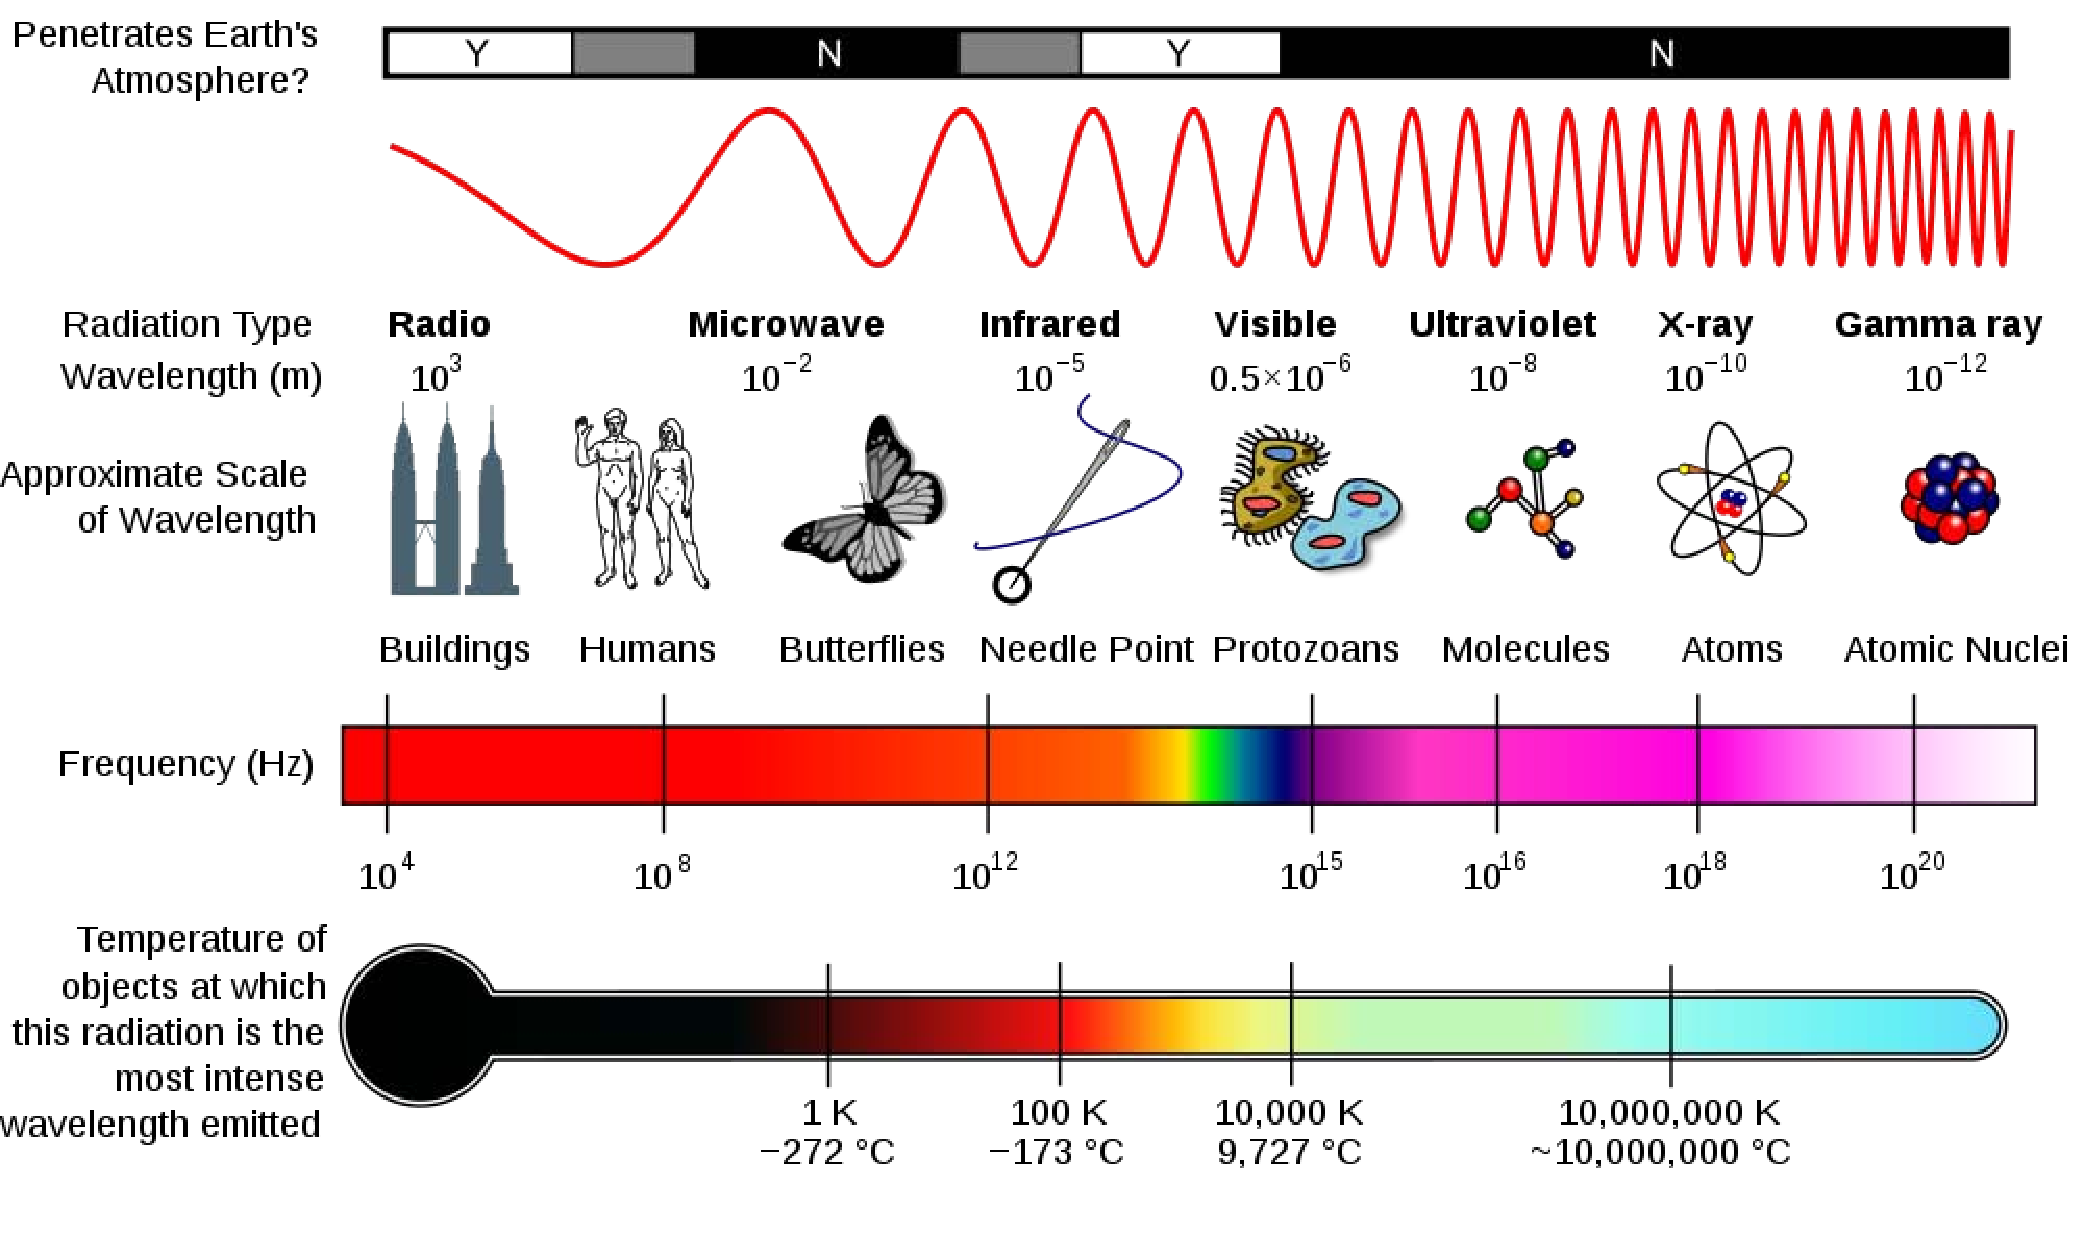
\includegraphics[width=11cm]{ch6/em_spectrum_properties} % ͼƬ�������Դ�Щ��ĸ��ͷ
  \end{center}
\end{figure}

\end{frame}

%%%%%%%%%%%%%%%%%%%%%%%%%%%%%%%%%%%%%%%%%%%%%%%%%%%%%%%%%%%%%%%%%

\begin{frame}% [shrink]
\frametitle{\textsc{Opacity of the Atmosphere}}

\begin{figure}
  \begin{center}
    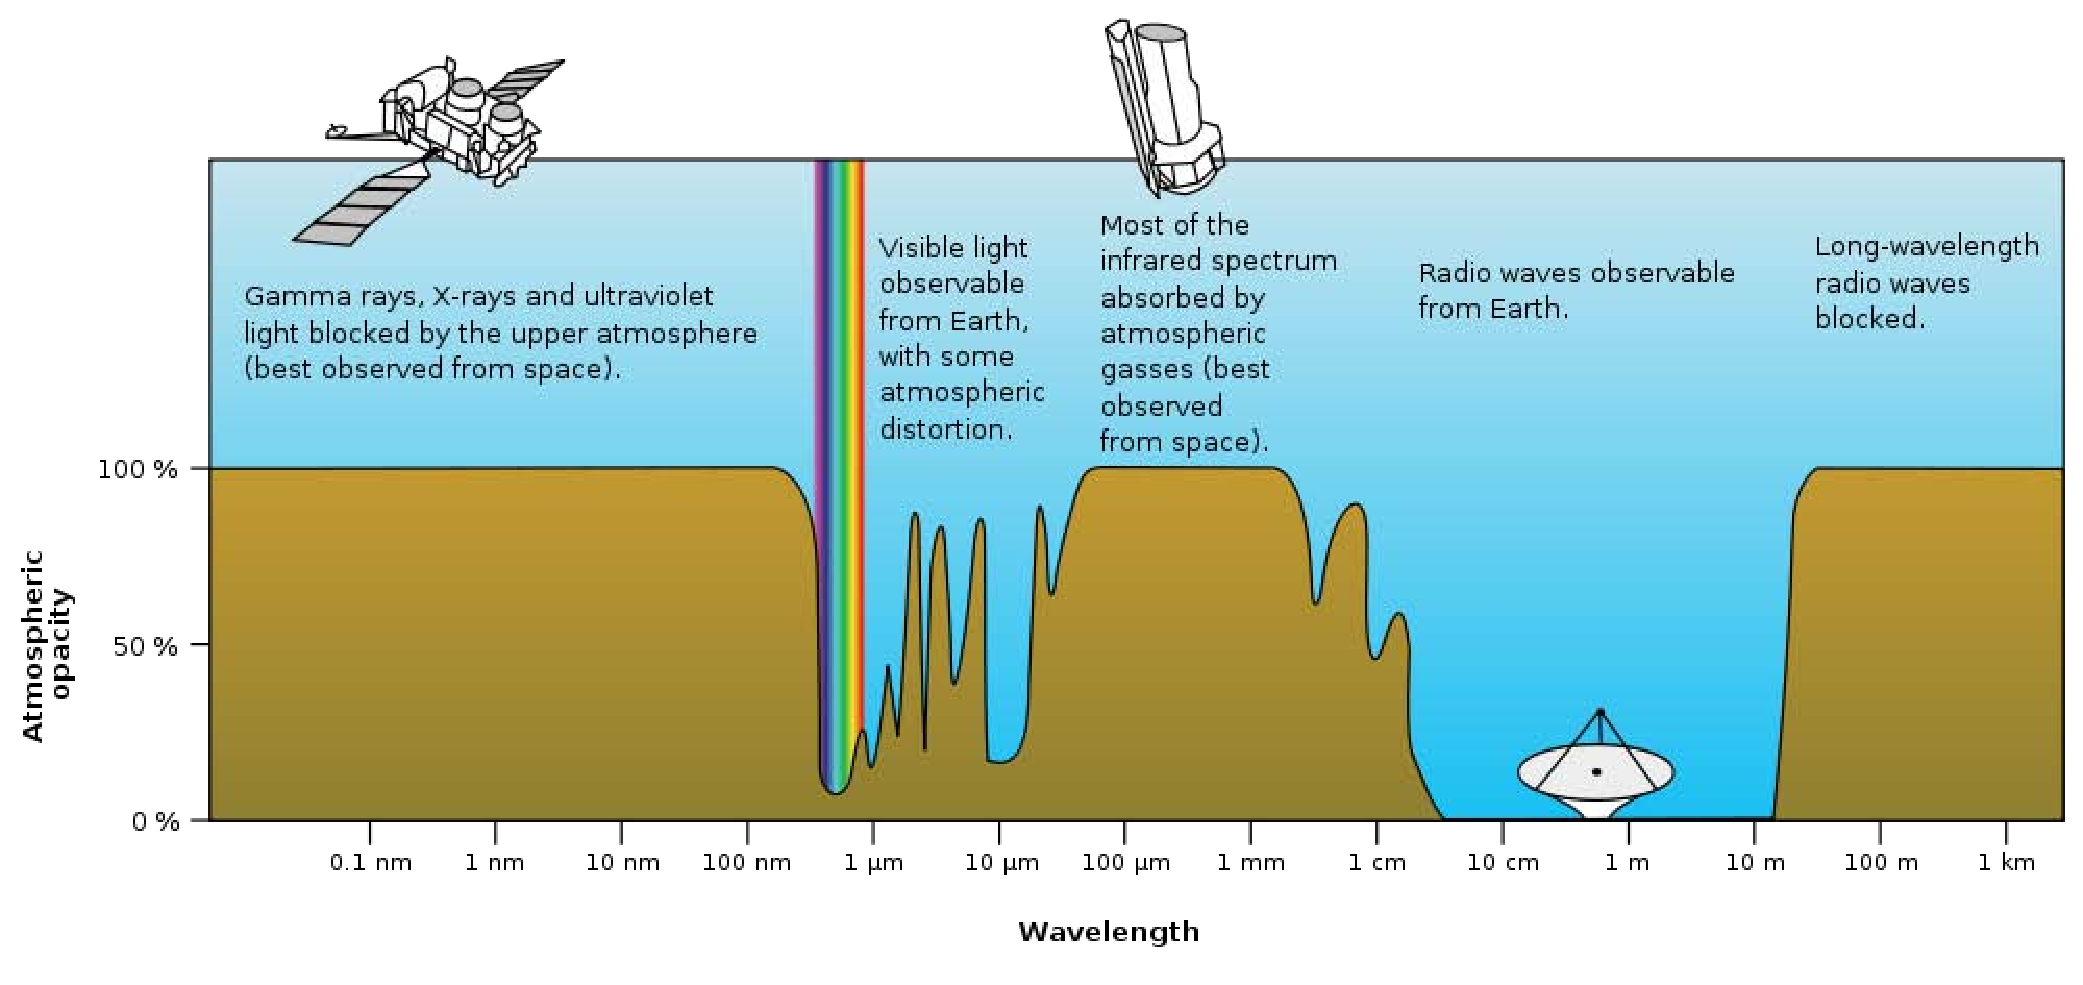
\includegraphics[width=11cm,height=6cm]{ch6/atmospheric_electromagnetic_opacity} % ͼƬ�������Դ�Щ��ĸ��ͷ
  \end{center}
\end{figure}

\end{frame}

%%%%%%%%%%%%%%%%%%%%%%%%%%%%%%%%%%%%%%%%%%%%%%%%%%%%%%%%%%%%%%%%%

\begin{frame}% [shrink]
\frametitle{\textsc{Main Mode of Radio Propagation}}

\hilite<1>Wave of certain frequency and polarization matches medium
with specific conditions, and will have a dominant mode of
transmission.һ��Ƶ�ʺͼ����ĵ粨���ض�ý��������ƥ�䣬������ij��ռ���ƵĴ�����ʽ��\pause

\hilite<2>Generally, radio waves propagate in the following modes:
\begin{itemize}%{enumerate}[<+->]
\item\hilite<2> Surface modes (ground wave)
\item\hilite<2> Ionospheric modes (sky wave)
\item\hilite<2> Direct modes (line-of-sight)
\item\hilite<2> Tropospheric modes
\end{itemize}%{enumerate}

\end{frame}

%%%%%%%%%%%%%%%%%%%%%%%%%%%%%%%%%%%%%%%%%%%%%%%%%%%%%%%%%%%%%%%%%

\begin{frame}
\frametitle{\textsc{Free space propagation}}



\rightline{\hyperlink{sec:6}{\beamerreturnbutton{back}} }
\end{frame}

%%%%%%%%%%%%%%%%%%%%%%%%%%%%%%%%%%%%%%%%%%%%%%%%%%%%%%%%%%%%%%%%
\subsection[Surface modes (groundwave) ���沨����]{Surface modes}\label{subsec:6-2}
%%%%%%%%%%%%%%%%%%%%%%%%%%%%%%%%%%%%%%%%%%%%%%%%%%%%%%%%%%%%%%%%

\begin{frame}
\frametitle{\textsc{Surface modes}}


\rightline{\hyperlink{sec:6}{\beamerreturnbutton{back}} }
\end{frame}

%%%%%%%%%%%%%%%%%%%%%%%%%%%%%%%%%%%%%%%%%%%%%%%%%%%%%%%%%%%%%%%%
\subsection[Ionospheric modes (skywave) �첨����]{Ionospheric modes}\label{subsec:6-3}
%%%%%%%%%%%%%%%%%%%%%%%%%%%%%%%%%%%%%%%%%%%%%%%%%%%%%%%%%%%%%%%%

\begin{frame}
\frametitle{\textsc{Ionospheric modes}}


\rightline{\hyperlink{sec:6}{\beamerreturnbutton{back}} }
\end{frame}

%%%%%%%%%%%%%%%%%%%%%%%%%%%%%%%%%%%%%%%%%%%%%%%%%%%%%%%%%%%%%%%%
\subsection[Direct modes (line-of-sight) �Ӿഫ��]{Direct modes}\label{subsec:6-4}
%%%%%%%%%%%%%%%%%%%%%%%%%%%%%%%%%%%%%%%%%%%%%%%%%%%%%%%%%%%%%%%%

\begin{frame}
\frametitle{\textsc{Direct modes}}


\rightline{\hyperlink{sec:6}{\beamerreturnbutton{back}} }
\end{frame}


%%%%%%%%%%%%%%%%%%%%%%%%%%%%%%%%%%%%%%%%%%%%%%%%%%%%%%%%%%%%%%%%
\subsection[Tropospheric modes ������ɢ�䴫��]{Tropospheric modes}\label{subsec:6-5}
%%%%%%%%%%%%%%%%%%%%%%%%%%%%%%%%%%%%%%%%%%%%%%%%%%%%%%%%%%%%%%%%

\begin{frame}
\frametitle{\textsc{Tropospheric modes}}


\rightline{\hyperlink{sec:6}{\beamerreturnbutton{back}} }
\end{frame}

%\include{data/pub}
%\include{data/ack}

%  »»Ò³¶¯Ì¬Ð§¹û:
%\transblindshorizontal<1> %  ˮƽ°ÙÒ¶´°Ð§¹û
%\transblindsvertical<2> %  ÊúÖ±°ÙÒ¶´°Ð§¹û
%\transboxin<3> %  ´ÓÖÐÐĵ½ËĽÇ
%\transboxout<4> %  ´ÓËĽǵ½ÖÐÐÄ
%\transdissolve<5> %  ÈܽâЧ¹û
%\transglitter<6> %  ÉÁ˸
%\transsplitverticalin<7> %  Êúֱ˺¿ª(ÏòÄÚ)
%\transsplitverticalout<8> %  Êúֱ˺¿ª(ÏòÍâ)
%\transsplithorizontalin %  ˮƽ˺¿ª(ÏòÄÚ)
%\transsplithorizontalout %  ˮƽ˺¿ª(ÏòÍâ)
%\transwipe<9> %  ͿĨ
%\transduration<10>{1} %  ½¥³ö

%%%%%% Latex ÉèÖÃ×ÖÌå %%%%%%

%ÏÔʾֱÁ¢Îı¾£º     \textup{Îı¾}
%Òâ´óÀûбÌ壺       \textit{ÃÀÔª·ûÎı¾ÃÀÔª·û}
%slantedбÌ壺      \textsl{Îı¾}
%ÏÔʾСÌå´óдÎı¾£º \textsc{Îı¾}
%ÖеÈȨÖØ£º         \textmd{Îı¾}
%¼Ó´ÖÃüÁ         \textbf{Îı¾}
%ĬÈÏÖµ£º           \textnormal{Îı¾}

%Latex ÉèÖÃ×ÖÌå´óСÃüÁîÓÉСµ½´óÒÀ´ÎΪ£º \tiny \scriptsize
%\footnotesize \small \normalsize \large \Large \LARGE \huge \Huge

% ³¬Á´¼°°´Å¥
%\hyperlink{sec:1}{\beamerreturnbutton{back}}
% \beamerskipbutton, \beamerbutton, \beamergotobutton, ºÍ \beamerreturnbutton

%%%%%%%%%%%%%%%%%%%%%%%%%%%%% »·¾³ %%%%%%%%%%%%%%%%%%%%%%%%%%%%%%%%%%%%%
%\begin{definitin} % ¿ÉÑ¡µÄ»¹ÓУºtheorem, lemma, corollary, proposition, example, proof
%  ¶¨ÒåµÄÀý×Ó¡£
%\end{definition}


\end{document}
